\documentclass[notoc, symmetric, nobib, nols]{towcenter-guideto-book}

\hypersetup{colorlinks, hyperfootnotes=true}% uncomment this line if you prefer colored hyperlinks (e.g., for onscreen viewing)

%uncomment to remove hyperlinks for Lulu upload
%\hypersetup{draft}

% creating an "ignore" command to deal with emdash problem \& comments in general
\newcommand{\ignore}[1]{}
\widowpenalty=10000

\usepackage[T1]{fontenc}
\usepackage[at]{easylist}
%\usepackage[utf8]{inputenc}
\usepackage{textcomp}
\usepackage[american]{babel}
\usepackage[autostyle]{csquotes}
\usepackage{endnotes}
\usepackage[strict]{changepage}
\usepackage{enumitem}
\setlist{noitemsep}
\usepackage{wrapfig}

\usepackage[notes15,strict,backend=biber,autolang=other,%
bibencoding=latin1,notetype=endonly,ibidtracker=constrict]{biblatex-chicago}
\bibliography{Citations.bib}
%\addbibresource{ChatAppsReadings.bib}
\usepackage{ifthen}
\usepackage{setspace}

\renewcommand*{\biburlsetup}{%
  \Urlmuskip=0mu plus 2mu\relax
  \mathchardef\UrlBreakPenalty=200\relax
  \mathchardef\UrlBigBreakPenalty=100\relax
  \mathchardef\UrlEmergencyPenalty=9000\relax
  \appto\UrlSpecials{%
    \do\0{\mathchar`\0\penalty\UrlEmergencyPenalty}%
    \do\1{\mathchar`\1\penalty\UrlEmergencyPenalty}%
    \do\2{\mathchar`\2\penalty\UrlEmergencyPenalty}%
    \do\3{\mathchar`\3\penalty\UrlEmergencyPenalty}%
    \do\4{\mathchar`\4\penalty\UrlEmergencyPenalty}%
    \do\5{\mathchar`\5\penalty\UrlEmergencyPenalty}%
    \do\6{\mathchar`\6\penalty\UrlEmergencyPenalty}%
    \do\7{\mathchar`\7\penalty\UrlEmergencyPenalty}%
    \do\8{\mathchar`\8\penalty\UrlEmergencyPenalty}%
    \do\9{\mathchar`\9\penalty\UrlEmergencyPenalty}}%
  \def\UrlBreaks{%
    \do\.\do\@\do\/\do\\\do\!\do\_\do\|\do\;\do\>\do\]\do\)\do\}%
    \do\,\do\?\do\'\do\+\do\=\do\#\do\$\do\&\do\*\do\^\do\"}%
  \def\UrlBigBreaks{\do\:\do\-}}
\usepackage{url}
%\setcounter{biburllcpenalty}{7000}
%\setcounter{biburlucpenalty}{8000}
\urlstyle{rm}
\appto\bibsetup{\sloppy}
%\appto\biburlsetup{\Urlmuskip=0mu plus 4mu\relax}
\setlength{\dimen\footins}{9.5in}
\renewcommand{\notesname}{}


\geometry{a5paper,left=0.6in,right=0.6in,top=0.6875in,headsep=\baselineskip,
textwidth=4.4in,textheight=6.83in,headheight=\baselineskip,marginparwidth
=.1in, marginparsep=0.1in}
%\geometry{a5paper,left=13mm,top=15mm,headsep=1\baselineskip,textwidth=
%122mm,textheight=185mm,headheight=\baselineskip,marginparwidth=10mm,
%marginparsep=5mm}
%%
% Adding setspace to tighten leading on margin notes
\usepackage{setspace}

%%
% Adding back marginnote functionality that I've stripped from tufte-common.def in the process of creating towcenter-common.def
\usepackage{marginnote}
\renewcommand{\marginnote}[1]{{\marginpar{\raggedright\footnotesize
\setstretch{1.025}%
#1}}}

%%
% Setting the footnote style to roman numerals in this case
\renewcommand{\thefootnote}{\roman{footnote}}

% more on bullet positioning: http://tex.stackexchange.com/questions/78167/indentation-within-an-itemized-list
% \setlist[itemize,1]{leftmargin=\dimexpr 26pt-.5in}


%%
% Resetting the footnote counter every page for clarity (I think)
%\usepackage{perpage} %the perpage package
%\MakePerPage{footnote} %the perpage package command

%%
% Resetting footnote counters every section?!
\makeatletter
\@addtoreset{footnote}{section}
\makeatother



%%
% Book metadata
\title{Guide to Podcasting}
\author{Vanessa Quirk - vquirk}
\publisher{Tow Center for Digital Journalism}


% use fontspec package and set titles to Georgia
\usepackage{fontspec}
\newfontfamily\titlefont{Times}
\newfontfamily\towknightfont{News Gothic MT}
%\newfontfamily\bodyfont{Caslon Regular}
\newfontfamily\frankmedium{Franklin Gothic Medium}
%\newfontfamily\frankregular{Franklin Gothic Regular}
%\newfontfamily\frankdemi{Franklin Gothic Demi}

%\setmainfont{Caslon Regular}

% add color package and define appropriate blues for title page
\usepackage{color}
\definecolor{darkblue}{RGB}{30,69,132}
\definecolor{lightblue}{RGB}{154,196,219}

% framed helps with graphics
\usepackage{framed}

% suppresses names and figure numbers on graphics
\usepackage{etoolbox}
\makeatletter
\patchcmd{\@caption}
  {\noindent\csname fnum@#1\endcsname: \ignorespaces}
  {}
  {}{}
\makeatother

%%
% Just some sample text
\usepackage{lipsum}

%%
% For nicely typeset tabular material
\usepackage{booktabs}

%%
% For graphics / images
\usepackage{graphicx,caption}
\setkeys{Gin}{width=\linewidth,totalheight=\textheight,keepaspectratio}
\graphicspath{{graphics/}}

% The fancyvrb package lets us customize the formatting of verbatim
% environments.  We use a slightly smaller font.
\usepackage{fancyvrb}
\fvset{fontsize=\normalsize}

%%
% Prints argument within hanging parentheses (i.e., parentheses that take
% up no horizontal space).  Useful in tabular environments.
\newcommand{\hangp}[1]{\makebox[0pt][r]{(}#1\makebox[0pt][l]{)}}

%%
% Prints an asterisk that takes up no horizontal space.
% Useful in tabular environments.
\newcommand{\hangstar}{\makebox[0pt][l]{*}}

%%
% Prints a trailing space in a smart way.
\usepackage{xspace}


% Prints the month name (e.g., January) and the year (e.g., 2008)
\newcommand{\monthyear}{%
  \ifcase\month\or January\or February\or March\or April\or May\or June\or
  July\or August\or September\or October\or November\or
  December\fi\space\number\year
}


% Prints an epigraph and speaker in sans serif, all-caps type.
\newcommand{\openepigraph}[2]{%
  %\sffamily\fontsize{14}{16}\selectfont
  \begin{fullwidth}
  \sffamily\large
  \begin{doublespace}
  \noindent\allcaps{#1}\\% epigraph
  \noindent\allcaps{#2}% author
  \end{doublespace}
  \end{fullwidth}
}

% Inserts a blank page
\newcommand{\blankpage}{\newpage\hbox{}\thispagestyle{empty}\newpage}

\usepackage{units}

% Typesets the font size, leading, and measure in the form of 10/12x26 pc.
\newcommand{\measure}[3]{#1/#2$\times$\unit[#3]{pc}}

% Macros for typesetting the documentation
\newcommand{\hlred}[1]{\textcolor{Maroon}{#1}}% prints in red
\newcommand{\hangleft}[1]{\makebox[0pt][r]{#1}}
\newcommand{\hairsp}{\hspace{1pt}}% hair space
\newcommand{\hquad}{\hskip0.5em\relax}% half quad space
\newcommand{\TODO}{\textcolor{red}{\bf TODO!}\xspace}
\newcommand{\ie}{\textit{i.\hairsp{}e.}\xspace}
\newcommand{\eg}{\textit{e.\hairsp{}g.}\xspace}
\newcommand{\na}{\quad--}% used in tables for N/A cells
\providecommand{\XeLaTeX}{X\lower.5ex\hbox{\kern-0.15em\reflectbox{E}}\kern-0.1em\LaTeX}
\newcommand{\tXeLaTeX}{\XeLaTeX\index{XeLaTeX@\protect\XeLaTeX}}
% \index{\texttt{\textbackslash xyz}@\hangleft{\texttt{\textbackslash}}\texttt{xyz}}
\newcommand{\towcenterbs}{\symbol{'134}}% a backslash in tt type in OT1/T1
\newcommand{\doccmdnoindex}[2][]{\texttt{\towcenterbs#2}}% command name -- adds backslash automatically (and doesn't add cmd to the index)
\newcommand{\doccmddef}[2][]{%
  \hlred{\texttt{\towcenterbs#2}}\label{cmd:#2}%
  \ifthenelse{\isempty{#1}}%
    {% add the command to the index
      \index{#2 command@\protect\hangleft{\texttt{\towcenterbs}}\texttt{#2}}% command name
    }%
    {% add the command and package to the index
      \index{#2 command@\protect\hangleft{\texttt{\towcenterbs}}\texttt{#2} (\texttt{#1} package)}% command name
      \index{#1 package@\texttt{#1} package}\index{packages!#1@\texttt{#1}}% package name
    }%
}% command name -- adds backslash automatically
\newcommand{\doccmd}[2][]{%
  \texttt{\towcenterbs#2}%
  \ifthenelse{\isempty{#1}}%
    {% add the command to the index
      \index{#2 command@\protect\hangleft{\texttt{\towcenterbs}}\texttt{#2}}% command name
    }%
    {% add the command and package to the index
      \index{#2 command@\protect\hangleft{\texttt{\towcenterbs}}\texttt{#2} (\texttt{#1} package)}% command name
      \index{#1 package@\texttt{#1} package}\index{packages!#1@\texttt{#1}}% package name
    }%
}% command name -- adds backslash automatically
\newcommand{\docopt}[1]{\ensuremath{\langle}\textrm{\textit{#1}}\ensuremath{\rangle}}% optional command argument
\newcommand{\docarg}[1]{\textrm{\textit{#1}}}% (required) command argument
\newenvironment{docspec}{\begin{quotation}\ttfamily\parskip0pt\parindent0pt\ignorespaces}{\end{quotation}}% command specification environment
\newcommand{\docenv}[1]{\texttt{#1}\index{#1 environment@\texttt{#1} environment}\index{environments!#1@\texttt{#1}}}% environment name
\newcommand{\docenvdef}[1]{\hlred{\texttt{#1}}\label{env:#1}\index{#1 environment@\texttt{#1} environment}\index{environments!#1@\texttt{#1}}}% environment name
\newcommand{\docpkg}[1]{\texttt{#1}\index{#1 package@\texttt{#1} package}\index{packages!#1@\texttt{#1}}}% package name
\newcommand{\doccls}[1]{\texttt{#1}}% document class name
\newcommand{\docclsopt}[1]{\texttt{#1}\index{#1 class option@\texttt{#1} class option}\index{class options!#1@\texttt{#1}}}% document class option name
\newcommand{\docclsoptdef}[1]{\hlred{\texttt{#1}}\label{clsopt:#1}\index{#1 class option@\texttt{#1} class option}\index{class options!#1@\texttt{#1}}}% document class option name defined
\newcommand{\docmsg}[2]{\bigskip\begin{fullwidth}\noindent\ttfamily#1\end{fullwidth}\medskip\par\noindent#2}
\newcommand{\docfilehook}[2]{\texttt{#1}\index{file hooks!#2}\index{#1@\texttt{#1}}}
\newcommand{\doccounter}[1]{\texttt{#1}\index{#1 counter@\texttt{#1} counter}}

% Generates the index
\usepackage{makeidx}
\makeindex

\begin{document}

% Front matter
\frontmatter

% r.1 blank page
\blankpage

% r.3 full title page
%\maketitle
%Using minipages to mimic existing layout for title page

%\cleardoublepage

\begin{figure}
\centering
\makebox[0pt][c]{%
\begin{minipage}[t][1\textheight]{0.2\textwidth}
\vspace{0pt}
\vfill

\includegraphics[width=.6\textwidth]{graphics/ColumbiaLogo.pdf}
\end{minipage}
\hfill
\begin{minipage}[t][1\textheight]{0.80\textwidth}
\vspace{0pt}
\begin{flushleft}

%\textcolor{darkblue}{\towknightfont{\fontsize{30}{30}\selectfont Guide to}}
\textcolor{lightblue}{\towknightfont{\fontsize{47}{47}\selectfont \textbf{Guide to}}}

\vspace{0.4in}

\textcolor{darkblue}{\textbf{\titlefont\fontsize{58}{58}\selectfont
Podcasting}}

\vspace{2.9in}
\textcolor{darkblue}{\towknightfont{\fontsize{16}{16}\selectfont \textbf{Vanessa Quirk}}}

\vspace{1.45in}

\textcolor{darkblue}{\towknightfont{\fontsize{7}{-3}\selectfont Tow Center for Digital Journalism\hspace{0.3in}Funded by the Tow Foundation and the\\[-0.08in]A Tow/Knight Guide \hspace{0.88in}James S. and John L. Knight Foundation}}
\end{flushleft}
\end{minipage}%
}%
\end{figure}



\blankpage
\blankpage
% v.4 copyright page


\null
\begin{fullwidth}
\noindent\textsf{\textbf{Acknowledgments}} \\[0.3cm]
\noindent\textit{Many thanks to Elizabeth Boylan, Pete Brown, Fergus Pitt, Benjamen Walker, Susan McGregor, and Emily Bell of the Tow Center for Digital Journalism for their support. Special thanks to Claire Wardle for generously giving me her time and fantastic feedback.
}\\[0.1cm]\noindent\textit{
Also thanks to all those who took the time to speak with me (on or off the record) for this project: Nick Quah (Panoply, Hot Pod), Robert S. Boynton (NYU), Tom Webster (Edison Research), Noah Shanok (Stitcher), Mark DiCristina (MailChimp), Jim Colgan (Audible), Brendan Monaghan (Panoply), Christa Scharfenberg (\textit{Reveal}), Rob Walch (Libsyn), Steve Nelson (Infinite Guest), Jenna Weiss-Berman (BuzzFeed), Clea Conner Chang (\textit{Intelligence Squared}), Jake Shapiro (PRX), Angela Stengel (First Run, ABC Radio), Kerri Hoffman (PRX), Hrishikesh Hirway (\textit{Song Exploder}), Erik Diehn (Midroll Media), Steve Wilson (Apple), Seth Lind (\textit{This American Life}), Parviz Parvizi (Clammr), Matt Lieber (Gimlet), Sarah van Mosel (New York Public Radio), Caitlin Thompson (Acast), Andy Bowers (Panoply), Jaclyn Friedman (Yes Means Yes), Mitra Kaboli (The Heart), Benny Becker (Israel Story), and Aaron Mahnke (\textit{Lore}).  
}\\[0.1cm]
\noindent\textit{\monthyear}
\end{fullwidth}
% r.5 contents
\tableofcontents


% r.7 introduction
\cleardoublepage


%%
% Start the main matter (normal chapters)
\mainmatter


\chapter{Executive Summary}

This report aims to explain why podcasts matter to digital journalism: as our world shifts to one of mobile consumption, podcasts represent a form of mobile-first content that engages with audiences in ways that no other mobile medium has previously.

This guide provides a detailed overview of the current podcasting landscape, which is characterized by industry disruption, new networks, increased podcast listening (especially on mobile devices), and heightened consumer awareness. As part of this overview, I describe the conceptual and technological challenges that podcasting must overcome if it is to achieve meaningful growth and industry legitimacy. I also briefly outline the challenges the industry faces as it looks to the future: the issues of iTunes as a gatekeeper, the short-term and long-term efficacy of networks, the ethical dilemmas that native ads and branded content pose, and the need for more creativity and diversity in content creation.

Podcasts are pursuing multiple revenue streams, including advertising/sponsorship, foundation support, direct support, subscription models, and live events. While advertising is currently the fastest-growing and most lucrative stream, these last three streams attempt to convert audience engagement and loyalty into recurring donations. 

Because there is no one-size-fits-all solution for generating revenue, and each podcast/company follows a different business model, it's important to consider the operational philosophies that inform how podcasts and networks raise revenue and prioritize revenue streams. This guide explores the myriad ways these philosophies play out in four case studies: PRX's \textit{Reveal}, Gimlet Media, BuzzFeed, and Panoply. 

It is still too early to declare any podcast or podcast company a ``success.'' Many podcasts/networks currently rely heavily on advertising and are still experimenting with alternative revenue streams. Outside of advertising and branded content, podcasts show the most potential as an audience engagement tool that can diversify content, add value to brands/consumers, and generate enthusiasm for direct support and/or freemium models. 

\chapter{Introduction}

\section{Podcasting: A Brief History}

In 1999, developers at Netscape had an idea for aggregating content from a variety of sites, so that readers would not have to visit their favorite sites individually to manually monitor the latest updates -- instead, the content would appear simply, \footnote{Although Lydon's show, \href{http://radioopensource.org/about/}{Radio Open Source}, is often credited as the first podcast (and his 2003 interview with Winer \href{http://blogs.harvard.edu/lydondev/2003/07/09/spoken-word-a-few-good-bloggers/}{the first podcast episode}), this claim is arguable as it depends upon one’s definition of podcasting. I have called ``Daily Source Code'' the first podcast because Curry's show included the software script that allowed for audio transfer to an mp3 device (which I am asserting is part of the definition of a podcast); Lydon's audioblog, while it included the enclosure that allowed for audio to be accessed via RSS, did not initially include this script.} in one place.\autocite{WhatisRSS} They launched a prototype and called it \href{https://en.wikipedia.org/wiki/RSS}{RDF Site Summary}.\autocite{RSSWiki} Today, this technology is known as RSS (Real Simple Syndication). 

In its original iteration, the RSS feed could only syndicate text. However, in 2000, developer and media personality, Adam Curry, approached software developer Dave Winer with an idea to adapt the feed so it could include larger media objects, such as mp3s. Winer developed just such a software -- and then another that could aggregate feeds from different sources. In early 2001, he used the nascent technology to aggregate songs by The Grateful Dead.\autocite{WINER}

In September 2003, while at Harvard University's Berkman Center, Winer showed the software to a fellow colleague, Christopher Lydon, a journalist who had been conducting in-depth audio interviews and inserting them as mp3s into his \href{http://blogs.harvard.edu/lydondev/}{blog} posts (Winer called it \href{http://scripting.com/davenet/2003/07/31/chrisLydonsWeblogForTheEar.html}{``A weblog for the ears''}\autocite{WINER2}). Once Lydon incorporated  Winer's technology, readers could subscribe to Lydon's blog and access the audio content automatically. One month later, a blogger named Harold Gilchrist referenced the blog when he hosted a session on ``audioblogging'' at the first ever BloggerCon, an annual conference that brought many central figures in the nascent blogosphere together.\autocite{Solutions}


Galvanized by Lydon's success, Adam Curry developed the prototype of software that allowed audio to be downloaded, passed to iTunes, and automatically transferred to mp3 players. To test it, Curry launched \textit{Daily Source Code}, arguably the first podcast, in August 2004.\footnote{See explanation in footnote above.}\autocite{Web2} A month later, Ben Hammersley, reporting for \textit{The Guardian}, suggested various possible monikers for the technology, including ``podcasting.''\autocite{Solutions} The next month, \textit{New York Times} reported that people were ``podcasting'' from the US to Australia to Sweden.{NYT2004} Indeed, in podcasting's early days, the hope was that the medium would be a revolutionary format, accessible to any amateur with a microphone and an internet connection, that would open up and democratize media. This is why, in keeping with this mission, the podcasting technology developed by Winer, Curry and others was purposefully kept open source and open access.\autocite{WINER}

In November 2004, at BloggerCon III, Adam Curry led a session, not on ``audioblogging,'' but \href{http://web.archive.org/web/20130729212422id_/http://itc.conversationsnetwork.org/shows/detail275.html}{``podcasting.''}\footnote{This section has been revised post-publication. Although the report originally stated Christopher Lydon was the first podcaster, it has been updated with more information regarding the technological definition of podcasting (see footnote 1). The change is not just technical; because Christopher Lydon was a professional radio journalist before he was a podcaster, attributing podcasting's beginnings to him fosters a narrative that podcasting has grown from radio. In fact, many other podcasts emerged around the same time as Lydon's and Curry's, and most were by non-radio professionals. \autocite{WINER}}\autocite{Solutions} That same month, the first podcast hosting platform, Libsyn, launched. In 2005, Public Radio International hosted its first daily news podcast, and TWiT (This Week in Tech), one of the first podcast networks, launched. Then, in June, \href{https://www.youtube.com/watch?v=K0KNLCbzZUw}{Steve Jobs announced on a stage in Silicon Valley} that podcasts, and indeed an entire podcast directory, would be available in iTunes 4.9.\autocite{JobsVideo} By December, the New Oxford American Dictionary declared ``podcast'' the word of the year.\autocite{PCHistoryWiki}

In 2006, podcasting continued to ride the coattails of the hype. \textit{The Ricky Gervais Show} became the most downloaded podcast in history. The first live podcast tour took place.\autocite{PCHistoryWiki} \textit{This American Life}, a weekly public radio program founded by Ira Glass in 1996, jumped on the bandwagon, making the show freely available as a podcast for the first time. Edison Research reported that \href{http://www.edisonresearch.com/the-podcast-consumer-2015/}{22 percent of Americans were aware of the term ``podcasting'' and 11 percent of the population had listened to a podcast at least once}.\autocite{EdPCconsumer}

Then the hype subsided. Podcasting went ``under the radar,'' so to speak, but it was growing slowly and steadily all the while. By 2014, Apple had one billion podcast subscribers. Edison Research reported that now \href{http://www.edisonresearch.com/the-podcast-consumer-2015/}{48 percent of all Americans knew the term podcasting and 30 percent had listened to a podcast before}.\autocite{EdPCconsumer} Then in October, \textit{This American Life} launched a spin-off show, one that would be released in installments, or serially, each week. They called it \textit{Serial}. 

\section{The So-Called Serial Effect}

Since \textit{Serial} was released, the narrative on podcasting has centered itself on a few cliché phrases: podcasting's ``back,'' in a ``renaissance,'' or a new ``golden age.'' There is no doubt, of course, that the show marked a watershed moment in podcasting history. It took \textit{This American Life} four years to reach a million downloads per episode; it took \textit{Serial} \href{http://longform.org/posts/longform-podcast-159-ira-glass}{four weeks}.\autocite{IraLongform} As of October 2015, the show has been \href{http://www.nytimes.com/2015/10/01/business/media/after-serial-what-podcasts-to-listen-to.html}{downloaded over 90 million times}.\autocite{NYTAfterSerial} 

However, few articles have been able to rigorously justify the ``renaissance'' moniker beyond \textit{Serial}'s success. First of all, podcasting metrics are notoriously murky, and thus it's difficult to pinpoint what podcasting \href{https://medium.com/@pete/downloads-listens-listeners-and-about-those-podcast-numbers-73a5ee3e2fca}{download numbers really mean in terms of listener numbers} (a single listener can download the same episode multiple times or across devices, inflating download data; plus, a download does not mean the downloader actually listened to the show).\autocite{DLvsListen} 

Secondly, many journalists covering this space overlook a vital factor in \textit{Serial}'s success: just a few weeks before the show's launch, Apple updated its mobile operating system, iOS, to include a native, undeletable podcast app. 

In all likelihood, this is why podcasting's first boom never fulfilled its initial promise of mainstream penetration: The technology (which required one to go to the iTunes store, download an episode, and then sync it to your device before you could listen on the go) was just too prohibitive. Apple's native podcast app, however, significantly lowered the barrier to entry for a great many consumers (as evidenced by the finding that Apple-device podcast downloads outpace Android downloads at a rate of \href{http://www.libsyn.com/wp-content/uploads/2015/06/PRLibsynNetGrowth021915Final.pdf}{5.4 to 1}).\autocite{libsyndata} Apple's latest system update, iOS 9, released in September 2015, further reduces the steps to access a podcast in the app. (In addition, it favors streaming; it takes one click to stream, two to download.) \textit{This American Life}'s Seth Lind predicts that the technology will continue to improve, eventually arriving at the point where podcasts, like music, become something listeners can easily and instantly access, rather than have to acquire.\autocite{lind} 

\begin{figure}
\begin{centering}
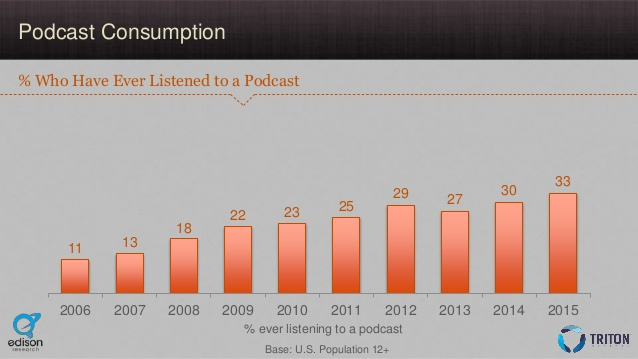
\includegraphics[width=.9\textwidth]{graphics/PODCAST15_EdPCconsumer_listened.jpg}
\caption\noindent{Figure 1: Percentage of Americans who have listened to a podcast from 2006 to 2015, via ``The Podcast Consumer 2015'' report, Edison Research.}
\end{centering}
\end{figure}

When \textit{Serial} launched, it was the perfect storm: fantastically reported, edge-of-your-seat content released just as for thousands of iPhone users podcasts were suddenly easier to find, subscribe to, and consume. Rob Walch, vice president of Libsyn, argued: ``The iPhone has done more for podcasting than anything else.''\autocite{Walch}

Thirdly, despite the fervent media attention, \textit{Serial} did not prompt a significant spike in overall listener growth for podcasts more generally. As Edison Research' The Podcast Consumer 2015'' report shows, although people are now listening to more podcasts, overall audience growth has remained slow and steady for the past decade. Today, a third of the American population has listened to a podcast at least once.\autocite{EdPCconsumer} However, these numbers are still nothing in comparison to terrestrial radio's: \href{http://www.nielsen.com/us/en/insights/reports/2015/state-of-the-media-audio-today-how-america-listens.html}{Over 91 percent of Americans listen to the radio each week}, and advertisers spend billions of dollars on radio each year (\href{http://www.statista.com/topics/1330/radio/}{radio is a 16-billion-dollar industry}).\autocites{nielsenradio, statistaradio} Podcasting is still far from meeting radio's dominance in terms of audience penetration or financial investment.

\begin{figure}
\begin{centering}
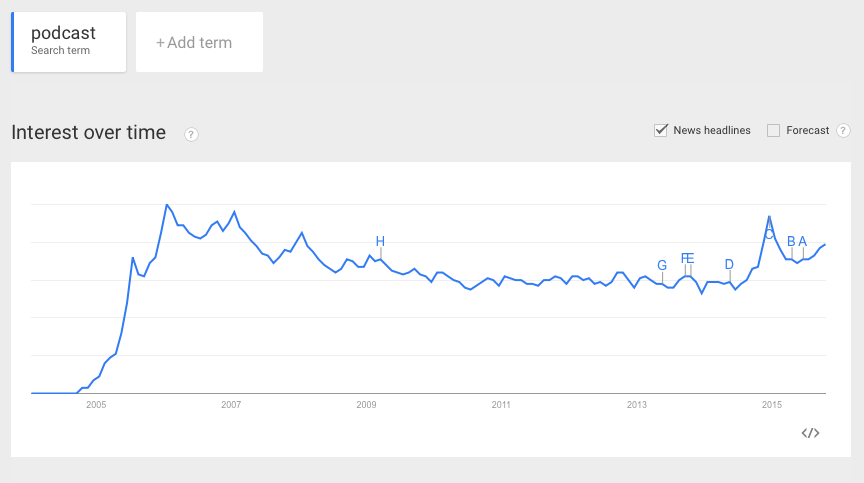
\includegraphics[width=.9\textwidth]{graphics/PODCAST15_Trends_podcast.png}
\caption\noindent{Figure 2: Frequency of ``podcast'' as a search term, from 2005 to 2015, via Google Trends.} 
\end{centering}
\end{figure}

So what has changed since \textit{Serial}? First, improved technology has made podcasts easier to consume. Second, \href{http://www.edisonresearch.com/the-podcast-consumer-2015/}{consumers are becoming more aware of podcasting as a concept}. Third, \href{http://www.edisonresearch.com/the-podcast-consumer-2015/}{those who already listen to podcasts are listening to more of them}, about six per week.\autocite{EdPCconsumer} Fourth, the media has begun to follow podcasting with more acute interest. And fifth, more and more individuals and media outlets are starting to enter the space. \href{http://www.libsyn.com/wp-content/uploads/2015/06/PRLibsynNetGrowth021915Final.pdf}{Libsyn reports} that more people signed up for new accounts in 2015 than ever before in the company's 11-year history.\autocite{libsyndata} Since launching in February 2015, \href{http://panoplymedia.tumblr.com/post/126958922613/eleven-shows-from-sports-illustrated-join-panoply}{Panoply has already acquired 20 partners} interested in launching podcasts of their own.\autocite{panoplyaudiometric} Debuting on October 12, WNYC Studios, a new podcasting division of WNYC, has similarly announced its partnerships with various authors, celebrities, and media outlets such as The New Yorker and VICE News.\autocite{wnycstudios} 

However, despite all the interest, few creators/outlets seem to know if podcasts can be economically viable. While many articles have focused on the potential of podcasting to grow audiences and earn revenue, there has been no comprehensive overview of how podcasts/networks are earning revenue today. The purpose of this guide is to do just that---to illustrate the state of the podcasting landscape in 2015, and to address the following central questions: Do podcasts generate revenue? How? What are the existing business models? And are they sustainable over the long term?

\chapter{Methodology}

The purpose of this report is to address the changes happening in the podcasting space, with a focus on the business side, and to answer the three following questions: 

\begin{enumerate}
\item What are the business models currently in operation?
\item To what extent have these business models proven successful?
\item Do these business models seem viable/resilient in the long term? 
\end{enumerate}

\noindent There is no one directory that includes all published podcasts available for study. The largest podcast directory is iTunes US; however, Apple has not published a dataset with this information. In June, I analyzed the Top 100 iTunes charts (cognizant that the top 100 does not mean the most downloaded, as iTunes rankings are sorted according to a private algorithm) and researched how each of these podcasts raises revenue. I did not, however, create a sufficiently large dataset from which I could draw overarching conclusions (for this type of analysis, I recommend you read sociologist \href{https://medium.com/@slowerdawn/how-podcasts-have-changed-in-ten-years-by-the-numbers-720a6e984e4e}{Josh Morgan's piece on Medium}\autocite{morgan}).

I built on this first phase of research by undertaking a review of the available literature, drawing particularly on industry reports such as Edison Research's ``\href{http://www.edisonresearch.com/the-infinite-dial-2015/}{The Infinite Dial 2015}'' and ``\href{http://www.edisonresearch.com/the-podcast-consumer-2015/}{The Podcast Consumer 2015},'' and Clammr's ``\href{http://www.slideshare.net/clammrapp/20150617-future-of-podcasting-2015-clammr-v-f}{Future of Podcasting 2015}.'' I also undertook a number of interviews with podcasting professionals, attempting to interview a wide variety of stakeholders involved in the business side of podcasting, including academics (NYU Professor Robert Boynton), market researchers (Edison Research's Tom Webster; Clammr's Parviz Parvizi), advertisers (MailChimp's Mark DiCristina), tech providers (Libsyn's Rob Walch; Acast's Caitlin Thompson; Stitcher's Noah Shanok), network executives, and content creators. 

As well as understanding its business, I wanted to investigate podcasting from the perspective of individual podcast creators and those networks which produce multiple podcasts. I devised an initial list of interviewees based on my spreadsheet of the Top 100 podcasts (choosing those that had particularly successful, interesting, or unusual revenue streams/trajectories). As I conducted these interviews, I employed a snowball sampling technique, asking participants to recommend other interview subjects, thereby expanding the list based on those recommendations. This list included representatives from individual shows (\textit{Reveal}, \textit{Intelligence Squared}, \textit{Song Exploder}) and the following networks/companies: Gimlet Media, Midroll Media, Panoply, Infinite Guest, Audible, BuzzFeed, PRX, the Australian Broadcasting Company, WBEZ, and New York Public Radio. Toward the end of my research, I sought out information from podcasters who could fill certain gaps in my research; for example, The Heart's Mitra Kaboli and Israel Story's Benny Becker answered an email inquiry about running live events, and Yes Means Yes's Jaclyn Friedman and \textit{Lore}'s Aaron Mahnke gave me insight into running podcasts without network support. 

Because this report gears toward a journalistic audience (both individuals interested in launching/sustaining podcasts and media outlets interested in pursuing podcasts), there are some significant, important subsets of the podcasting community that are conspicuously underrepresented---most notably comedy podcasts, talk radio podcasts, and self-help podcasts. 

I should also stress that this is a U.S.-centric report; because most media in the United States is privately funded, the expectations of consumer/foundational giving are substantially different than in countries with strong governmental support of media. Also, due to the fast-paced nature of this sphere, which changes on a daily basis, and the time required to publish, I should warn the reader that this report may be missing relevant information released after the final draft was submitted. 

\chapter{Why Podcasting Matters}

Podcasting's present and future, particularly its business models, are relevant to digital journalism for two major reasons. First, podcasting is a medium that lends itself to mobile consumption, and thus provides a means for reaching audiences in ways other media cannot. Second, podcasting offers a level of engagement with audiences that is incomparable with other digital media; it thus presents a remarkable opportunity for journalistic outlets to cultivate audience relationships and experiment with new forms of revenue generation.

\section{The Growth of Mobile}

\begin{figure}
\begin{centering}
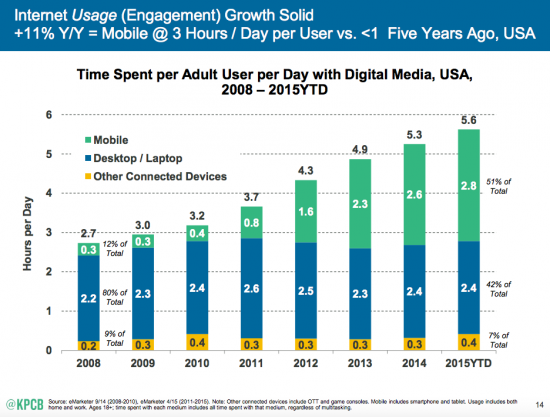
\includegraphics[width=.9\textwidth]{graphics/PODCAST15_KPCB_Mobile.png}
\caption\noindent{Figure 3: Time spent on mobile phones overtakes desktop usage in 2014. By KPCB, accessed via SmartInsights.com}
\end{centering}
\end{figure}

\href{http://www.smartinsights.com/internet-marketing-statistics/insights-from-kpcb-us-and-global-internet-trends-2015-report/}{According to a report on mobile technology trends from KPCB}, Americans now use their smartphones more than any other device to access the Internet---and it's a trend that appears to be on the rise.\autocite{KPCB} Similarly, mobile listening is by far the predominant method of podcast consumption today (63 percent of Libsyn-hosted podcasts were requested from mobile devices in 2014, up from 43 percent in 2012, according to \href{http://www.libsyn.com/wp-content/uploads/2015/06/PRLibsynNetGrowth021915Final.pdf}{Libsyn's internal data}), and it continues to grow month by month.\autocite{libsyndata} Podcasting should be considered a mobile-first medium.


As a mobile medium, podcasts have an advantage over text and video: They can be consumed in the moments when visual media consumption is inconvenient or impossible, like driving, commuting, exercising, doing housework, etc. Angela Stengel, digital product manager at ABC Radio, told me about an in-depth study in which ABC asked its listeners to explain the role that podcasts play in their lives. The study \textit{Reveal}ed that, unlike radio, podcasts serve two kinds of functions: either to keep listeners company in the home or office (in these cases, listeners prefer host-led, chat-based podcasts) or to ``transport them to another world'' (here, listeners prefer highly produced, story-based podcasts like \textit{Radiolab} or \textit{This American Life}). In either case, however, consumers are generally listening alone, from beginning to end, and engaging intimately with the material.\autocite{Stengel} 

\begin{figure}
\begin{centering}
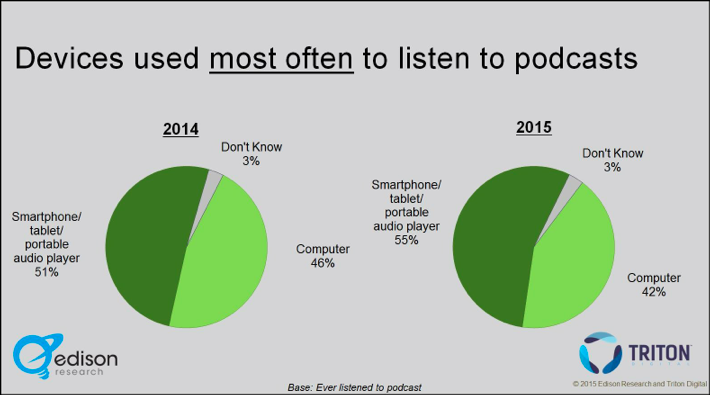
\includegraphics[width=.9\textwidth]{graphics/PODCAST15_EdInfinite_devices.png}
\caption\noindent{Figure 4: Podcast listening according to device. ``The Infinite Dial 2015,'' Edison Research.}
\end{centering}
\end{figure}

This is the kind of insight that podcast creators have long suspected instinctively, but have not had the research to support their claims. As Jenna Weiss-Berman, director of audio at BuzzFeed, told me: ``I don't think it's the kind of medium that lends itself to virality. It's not a one-minute video, and it's not an article you can quickly scroll through and look at the pictures and say you read it. You have to sit and engage.''\autocite{wb}

As such, podcasting offers an alternative vehicle for journalism: one which is easily accessible on mobile phones (where more and more consumers spend their time), privileged at certain hours of the day, and has the unique characteristic of eliciting consumers' close attention. 


\section{An Antidote to Advertising in the Internet Age?} 
At a time when consumers have become increasingly immune to display ads (Doubleclick currently measures global click-through rates on display ads at 0.06 percent), podcasts offer a potentially interesting vehicle for digital advertising.\autocite{ctr}

First, there's the engagement that podcasts inspire in listeners. Mark DiCristina explained that MailChimp likes podcast advertising because ``people are generally tuned into podcasts,'' and thus the ads are ``sticky.''\autocite{mailchimp} Sarah van Mosel commented: ``All these brands---regardless that we don't have standard measurements and that you can't track things---come back again and again and again because of the off-the-charts level of engagement podcasting has, that more than compensates for the lack of metrics.''\autocite{mosel}

Second, podcast listeners are loyal. They form relationships with hosts and return to shows regularly. In Caitlin Thompson's words: 

\begin{quote}
There's a regularity in listens. If you're The Huffington Post or BuzzFeed or Vox or Fusion, you can do a great job with reaching an audience with one particular piece of content, but it's really hard to guarantee that they're going to come back. That's why you have monthly visitors versus unique visitors, and you want to have a healthy proportion of that, because you want to be attracting new people but you also want to be retaining others so your advertisers see that they know what they're reaching.\autocite{thompson} 
\end{quote}

Third, surveys suggest that podcasts, which typically have host-read ads, don't engender advertising aversion.\autocite{wolfdenraphael} Two caveats here: one, survey-takers complete surveys voluntarily, and so generally represent the opinions of the keenest listeners; and, two, as \href{http://www.vox.com/2015/9/28/9408375/podcast-ads}{Vox's Philip Edwards} pointed out, podcasts have become oversaturated with the same ads, which can be annoying---especially since they're difficult to skip.\autocite{voxphil} Nevertheless, Mark DiCristina has found that: 

\begin{quote}
People typically don't mind the ads because they're read by the hosts and integrated into the content in a way that's more natural than in other mediums [...] there's a transference of credibility that happens there.\autocite{mailchimp}
\end{quote}

Those podcasters unrestricted by the FCC guidelines that constrain public radio have been further experimenting with means of integrating ads into content in innovative and entertaining ways. Comedy podcasts like \href{http://nerdist.com/podcasts/nerdist-podcast-channel/}\textit{The Nerdist} and \textit{\href{http://www.wtfpod.com}{WTF with Marc Maron}}, whose quick-witted hosts work the ad copy into their conversations, are particularly successful at this. Most prominent in this field, however, is Gimlet Media, which sells its native ads as ``the best mobile ad unit[s] in existence'' (more on this in the Gimlet case study below).\autocite{lieber}

Obviously, these ads are digital. As technology improves and progresses, podcast ads could one day offer the tracking capabilities and data that online ads do currently. In the meantime, podcast ads certainly offer an intriguing alternative to advertisers hoping to reach and engage with digital, mobile consumers. As such, they could represent a paradigm shift in the way we conceptualize advertising in the 21st century. Sarah van Mosel explained: 

Maybe scale is a very 20th-century way of looking at advertising. I think the most amazing experiences are customized just for you. Millennials aren't jaded about marketing, they just have high expectations for authenticity and customization---and they should.\autocite{mosel}

\chapter{Where We Are Today} 

Creators are fond of describing podcasting as still in its ``Wild West'' stage, a time when the rules haven't been formulated (let alone enforced) and everyone is---in terms of content, metrics, advertising rates, and business models---flying blind. 

This concept underplays the extent to which podcasting technology, storytelling, and revenue creation has evolved since its emergence in the early 2000s. Second, it elides the legacy of radio upon podcasting, most particularly the strong influence of both talk radio and public radio on its formats and revenue streams. 

On the level of distribution and production, podcasting has unquestionably disrupted radio, hurtling the major players into a state of flux. Whereas local stations once relied on major distributors such as NPR for content, and producers were equally dependent upon them for reaching large audiences, the digitization of audio has rendered traditional distributors unnecessary. PRX, the public radio exchange, has pivoted from a station marketplace into an online platform where producers can upload their work directly for stations to download. What's more, stations are no longer the only outlets for creators; creators can share their podcasts on a variety of platforms, some of which allow them to reach audiences and earn revenue directly.

``We're in a position where every producer can also be a distributor if they want,'' Seth Lind, director of operations at \textit{This American Life}, explained. ``There's kind of an identity crisis, and this is happening at the public radio station level, too. It's like, `Are we producers? Are we distributors? Do we need distributors?'''\autocite{lind}

Distributors, even the public radio behemoths like NPR, have lost their centrality in the audio ecosystem. \textit{This American Life}, although still distributed on public radio, has become an \href{http://current.org/2015/07/ira-glass-starts-own-company-for-this-american-life-serial/}{independent, public benefit corporation}, allowing it to maintain direct relationships with advertisers.\autocite{talpbc} Instigated by growing advertiser interest, and the need to bundle shows to maximize impressions, new podcast networks like Gimlet Media and Midroll Media have emerged, promising producers greater editorial freedom, higher salaries, or both. Almost weekly, individuals are leaving the public radio system to join them. Just this October, WNYC announced the creation of WNYC Studios, a podcast division that will self-distribute, raise money to develop programming, and hopefully incentivize talent to remain within the company.\autocite{wnycstudios}

Despite the uncertainty rife within the space, podcasting is making significant strides toward mainstream legitimacy as an industry. Central to this acceptance, of course, is achieving a critical mass of listeners. All interviewees discussed this fact: Podcasts need bigger audiences. 

Public radio was able to grow its audience size by giving away high-quality content for free and then monetizing that audience via sponsorship and fundraising. Podcasts have inherited that mantra: Content first, money later. In the words of Stitcher co-founder Noah Shanok: ``The single biggest inhibitor in terms of revenue is audience size. As soon as the audience is there, dollars will follow.''\autocite{shanok} Seth Lind put it another way: ``It's sort of like an `if they come, we will build it' business model.''\autocite{lind}

However, unlike public radio, podcasts are an on-demand medium. As Panoply's chief content officer, Andy Bowers, explained: Radio and podcasting are ``cousins, they're not even siblings.'' Podcasts are ``impossible to listen to by accident. Each time it's a choice. Radio is more laidback; you pick stations and program them in and you float around. You don't have to make a choice.'' He added, ``It's harder to get people to do that [to make that choice], but once you get them, they tend to stay around, like they've joined a club.''\autocite{bowers}

To reiterate Bowers's point, ``once you get them, they tend to stay around.''\autocite{bowers} However, the ``getting them'' remains the challenge at hand, and podcasting still has significant barriers obstructing its audience growth.

\section{Podcasting's Barriers to Growth}

Despite the work that \textit{Serial} has done to make podcasting better known among the public, the concept of podcasting remains foreign to many listeners. Indeed, it could be argued that podcasting remains in an ``early adopter phase.'' A \href{http://awesome.midroll.com}{Midroll white paper shows that 67 percent of podcast listeners are 18--34} (to compare, only 30.2 percent of radio listeners fall in this demographic).\autocite{midrollpaper} The podcasting audience skews toward the under-40s, a generation for whom the concept of on-demand content makes sense. 

Clea Conner Chang, the director of marketing for \textit{Intelligence Squared}, described the issue as a branding problem: 

People say, ``What's a podcast? How do I get a podcast?'' It has an inherent branding problem. [...] It's just radio on demand. You can hear your favorite show any time, and they just don't realize how it works yet, how convenient it is. It wasn't until a couple of years ago that streaming video became something with mass appeal, and this is streaming audio. It still hasn't made that association. [...] Podcasting is on this precipice of being something understood by the masses---it's not there yet.\autocite{chang} 

Closely related to the conceptual problem of podcasting (what is a podcast?) is the technical problem (how do I get a podcast?). Mark DiCristina, the marketing director for MailChimp (a company that advertises on a variety of popular podcasts, including \textit{Serial}), explained the problem: ``People still have to learn how to find podcasts. The whole concept of podcasting is still hard for some people to get their heads around. The technology will get better and there will be easier ways to consume and find podcasts, but right now there's still a barrier.''\autocite{mailchimp} 

One attempt to overcome this problem and promote podcasting's cross-generational appeal is Ira Glass's ``How to Listen to a Podcast''video, in which he and his elderly neighbor explain how accessible podcasts really are.\autocite{iramary} 

\begin{figure}
\begin{centering}
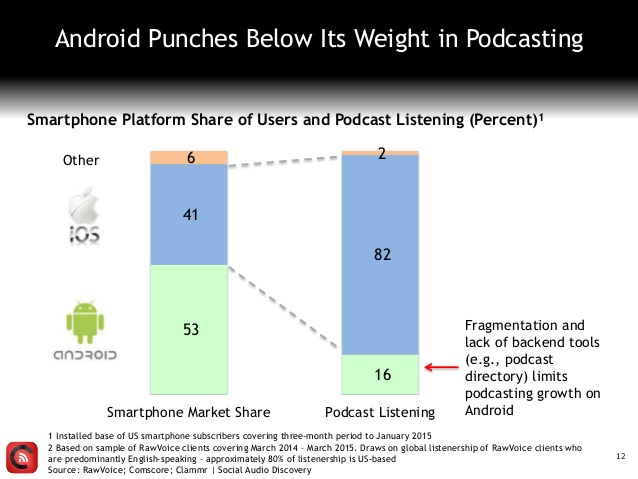
\includegraphics[width=.9\textwidth]{graphics/PODCAST15_clammrfuture_android.jpg}
\caption\noindent{Figure 5: iOS users account for over 80 percent of podcast listening, Android users for just 16 percent. Clammr ``Future of Podcasting 2015'' report.}
\end{centering}
\end{figure}

Moreover, while podcast listening remains strong on iOS, and Apple's native podcast app continues to improve, Android users---whose numbers are far greater than iPhone owners (one billion versus 470 million)---remain an untapped audience for whom podcast listening remains difficult.\autocite{smartphones} Apple device podcast downloads outpace Android downloads at a rate of \href{http://www.libsyn.com/wp-content/uploads/2015/06/PRLibsynNetGrowth021915Final.pdf}{5.4 to 1}.\autocite{libsyndata} Lind put it this way: ``This is a moment in podcasting [Google and Samsung are] not capitalizing on.''\autocite{lind} 

Although apps such as Stitcher have emerged to fill the gap for Android users, they don't compare to the ease of a native app. As Libsyn vice president Rob Walch pointed out, podcasting has been ``an Apple-centric media because Apple has been behind it to promote it. Android will never come close to iOS until Google installs a native player in Android.'' Indeed, to reach listeners on Android devices, Walch recommends that shows develop their own apps so that users can more easily search for and access their content.\autocite{Walch} 

\begin{figure}
\begin{centering}
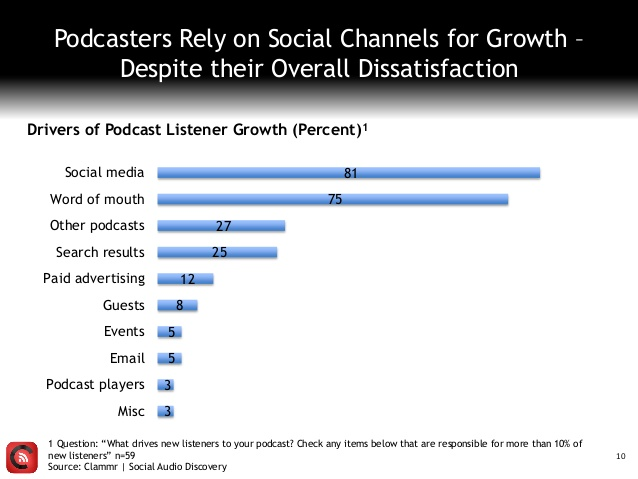
\includegraphics[width=.9\textwidth]{graphics/PODCAST15_clammrfuture_drivers.jpg}
\caption\noindent{Figure 6: Social media and word of mouth drive listeners to podcasts. Clammr ``Future of Podcasting 2015'' report.}
\end{centering}
\end{figure}

With or without an app, searching for podcasts remains somewhat difficult on iOS and Android alike. The same is true for discovering new podcasts. According to \href{http://www.slideshare.net/clammrapp/20150617-future-of-podcasting-2015-clammr-v-f}{Clammr's 2015 survey of podcasters}, cross-promotion on other podcasts, social media, and word of mouth remain the main ways listeners learn of new shows.\autocite{clammrfuture} Walch, who has over a decade of experience in the podcasting space, maintains that word of mouth will remain the most popular way podcasts are discovered and shared.\autocite{Walch} Others, such as Acast's Caitlin Thompson and Panoply's Andy Bowers, point to Netflix, which has successfully used algorithms to aid viewer discovery, as a potential reference point for podcasting's future.\autocite{thompson} \autocite{bowers}

Companies such as \href{http://www.clammr.com/}{Clammr} have emerged to try to make audio---a ``fundamentally not social'' technology in the words of Clammr CEO Parviz Parvizi---``easier to clip and share on social media.''\autocite{parvizi} Hosting platform \href{http://www.acast.com/}{Acast} includes a socially rich player as an incentive for podcasters to use its services. \href{https://www.popuparchive.com}{Pop-Up Archive} is transcribing podcasts in an effort to make them both easier to discover and share. A recent \href{http://audiohackathon.com/}{audio hackathon}, sponsored by \textit{This American Life}, similarly focused on ways that audio technology could enable more social listening experiences.\autocite{hotpodhackathon} 

Despite these early efforts, podcasting creators remain uncertain of the extent to which improved sharing and discovery tools are vital to podcasting's growth; far more important, as \textit{New York Magazine}'s Kevin Roose has pointed out, is the development of dashboard technology that will make podcasts easier to listen to in the car.\autocite{PCcars} 

Because \href{http://qz.com/195349/the-remarkable-resilience-of-old-fashioned-radio-in-the-us/}{almost half of radio listening happens in cars}, integrated dashboard technology---such as Apple's CarPlay and Google's Android Auto---could offer the key to unlocking audience growth.\autocite{radiocars} As Gimlet Media's Matt Lieber said, ``Until we have a mainstreamed solution to digital audio in cars, we're being held back.''\autocite{lieber} Most major automakers have already begun to integrate the technology into their latest models. \href{http://gizmodo.com/chevy-is-bringing-apple-carplay-and-android-auto-to-the-1707219276}{GM, for example, is aggressively adding Apple CarPlay to Chevrolets and Cadillacs}.\autocite{gm} A report from IT advisory firm \href{http://www.forbes.com/sites/samsungbusiness/2015/09/23/how-your-car-is-becoming-the-next-hot-tech-gadget/}{Gartner predicts that} ``by the end of 2020, 70 percent to 80 percent of all new vehicles in the United States will offer connected-car functionality.''\autocite{gartner} Of course, since consumers buy cars \href{http://www.forbes.com/sites/jimhenry/2012/01/20/average-car-in-the-u-s-now-over-10-years-old-a-record/}{every 11 years or so}, it will take about that time for radio consumers to convert into podcast listeners in significant numbers.\autocite{carbuying} 

\section{Metrics, Consumer Data, and Industry Standards}

Even though many platforms, such as SoundCloud and Acast (which both stream audio), have sophisticated analytics, the fact remains that the majority of podcasts are downloaded through iTunes (roughly 70 percent).\autocite{digiday} Once a podcast is downloaded, there is no way of knowing what happens to the file, how long it was listened to, how many times, or when. Moreover, since the subscribers ``belong'' to iTunes, creators have little knowledge of their listener demographics.

There are two camps in the podcasting sphere: One maintains that the tools of radio (surveys, extrapolations, etc.) are sufficient for podcasting measurement. The other wishes to push podcasting technology far enough to exploit the medium's full digital potential---to the point that everything is ``point to point measured,'' in the words of Sarah van Mosel.\autocite{mosel} 

Unlike online journalists, who have a plethora of statistics at their fingertips that allow them to make informed decisions about how to format and publish their content, podcasters have almost no idea how their audiences interact with their work. PRX CEO Jake Shapiro believes this kind of information would create ``a feedback loop for producers, so they know who their audience is, how they should craft their stories, what time of the day or the week they can release them.''\autocite{shapiro} Panoply's Nick Quah agreed: ``What did Chartbeat do for digital media? It ruined a lot of journalists' lives, because it's all they ever think about. We want to get to that level.''\autocites{quah, petre} 

Of course, improving metrics and data on consumers would also prove invaluable to another group: advertisers. As podcasting advertising begins to expand to include not just direct response advertising but also brand advertising, this information becomes all the more vital. Van Mosel explained: ``Branding people have a picture of the person they want to reach in their mind. You can get at it with surveys, but the Holy Grail, the next big step, is to figure out how to link back to the demographic and psychographic data that you can prove and then target to.''\autocite{mosel} 

Mark DiCristina, marketing director for MailChimp, put it this way: ``I would love to know all kinds of data: demographic data, age, gender, income, industry type, what they do for work, what percentage are in marketing or use email marketing. For now I've accepted that's not available any time soon.''\autocite{mailchimp}

Although advertisers like DiCristina have come to terms with limited consumer data for downloaded podcasts, there is, at least, some progress around better understanding listeners who stream podcasts. At WNYC, van Mosel has already overseen the conversion of ads into dynamic, programmatic ads, which can be continually trafficked into shows' back catalogues (where about 40 percent of listening occurs, vastly increasing ad impressions).\autocite{mosel} These ads also include tracking pixels that advertisers can use to ensure ads are delivering; as van Mosel explained, it's a ``lifeline to say `legitimacy is happening here.'''\autocite{mosel} Acast similarly injects trackable ads at point of play, and Panoply recently acquired the tech company Audiometric in order to offer a similar technology (for more on this, see the Panoply case study).

Another signal of podcasting's imminent exit from the Wild West is the emergence in the last six months of two separate podcasting upfronts (intended to inspire advertisers to sponsor upcoming content). Also notable is the creation of a working group at the Interactive Advertising Bureau, which aims to establish advertising standards. Many of the podcasters I spoke with recognized the need for an objective standard for audience measurement, one which all podcasters could agree to follow. Matt Lieber, president of Gimlet Media, suggested a reliable third party that will audit podcasting data, much as the Nielsen Ratings do for television, as a vital next step in legitimizing the podcasting industry.\autocite{lieber} 

\chapter{Revenue Streams}

As any media outlet in the 21st century is more than aware, diverse sources of revenue are necessary for long-term sustainability. Outlined below are four major sources from which podcasts and podcast networks generate revenue: advertising and sponsorship, direct support, foundation support, and membership/subscription models. Also mentioned are a few streams that, while generally less lucrative, are easy to implement or serve strategic purposes, such as live events and partnerships.

The division between these categories is somewhat arbitrary (what, in essence, distinguishes a wealthy individual's large donation from a foundation's small contribution?); however, I have borrowed these categories from interviewees who explicitly mentioned the following revenue streams in these terms. More important to note is that each podcast/network finds its own balance between these sources---some depend significantly on advertising while others maintain public radio's ``three-legged stool'' philosophy (in which three revenue sources---usually advertising, direct support, and foundation support---are conscientiously and purposefully given equal weight). 

\section{Advertising and Sponsorship}

For those I interviewed, advertising is currently podcasting's most lucrative and fastest-growing revenue stream. Advertisers have traditionally utilized podcasts for direct response ads (in which the host gives listeners a code or URL to receive a discounted service; these ads' success have allowed podcasts to charge high rates).\autocite{bowers} However, brand advertisers are becoming more prevalent. Although CPMs\footnote{See glossary for definition.} vary depending on audience quality and the level of host attention the ad receives, podcast advertising is, according to DiCristina, remarkably cost-effective compared to advertising in other media.\autocite{mailchimp}

\section{Direct Support}

From the beginning, podcasts have leveraged their direct audience relationships by asking for listener support via donations or pledges. Taking a cue from public radio, the Maximum Fun network does \href{http://www.maximumfun.org/donate}{yearly pledge drives and has a tiered membership model, for example}.

Jake Shapiro foresees direct support happening in innovative ways in the future, as PRX (and podcasts in general) seeks to convert ``passionate fan support into a more sustained way of long-term contributing.''\autocite{shapiro} \href{https://www.patreon.com/}{Patreon}, a site that allows consumers to regularly support creators, has become a popular option for many podcasters. Although not meant for listener donations per se, the \textit{StartUp} \href{http://www.wearehearken.com}{Hearken} provides media outlets with \href{http://knightfoundation.org/blogs/knightblog/2015/7/27/curious-city-inspires-scalable-model-engagement-journalism-answers-peoples-questions/}{listener support modules that allow listeners to engage with the creation process from inception to publication} (which could potentially make listeners more amenable to contributing financially). Kickstarter has been used to fund specific goals around launching new podcasts or funding new seasons, as well. \href{http://radioambulante.org}{Radio Ambulante} was one of the first to have success with Kickstarter; in early 2012, about a year into the project, it \href{https://www.kickstarter.com/projects/1255653356/radio-ambulante/description}{raised 46,032 dollars} (just over its 40,000-dollar goal).\autocite{ambulante}

PRX has also seen marked success with Kickstarter campaigns. In August of 2012, Roman Mars hoped to earn 42,000 dollars for the third season of his popular show 99\% Invisible, distributed by PRX. He used both challenge grants and stretch goals to incentivize donors. In the end, he \href{http://current.org/2012/08/podcast-with-limited-radio-airplay-sets-kickstarter-record/}{raised over 170,000 dollars}.\autocite{mars} In November of 2014, PRX and Mars turned again to Kickstarter to fund their podcast collective/network Radiotopia, hoping to raise 250,000 dollars. They \href{http://knightfoundation.org/blogs/knightblog/2014/11/14/radiotopia-sets-record-for-publishing-and-radio-funding-on-kickstarter/}{raised 620,412 dollars} and became the most-funded radio/podcast project in Kickstarter history.\autocite{radiotopia}

However, while Kickstarter is a tremendous opportunity to raise both funds and media attention, it's by no means a sure bet. A brief glance at the Kickstarter audio and radio/podcast pages shows dozens of Kickstarter ventures that failed to attain their goals. A successful Kickstarter campaign requires strategic and time-intensive marketing initiatives.

\section{Foundation Support}
Not-for-profit podcasts in particular have found success in cultivating grants from foundations that align with the podcast's content or mission. For example, Radiotopia was awarded a \href{http://www.niemanlab.org/2015/05/knight-foundation-invests-1-million-in-creator-driven-podcast-collective-radiotopia/}{one-million-dollar grant from the Knight Foundation} in May to develop new shows and reach new audiences.\autocite{million} Of course, grant money often comes with strings attached; foundations generally give money on the condition that content producers cover certain topics/issues.
 
\section{Membership, Subscription, or Premium Models}

Many podcasts and podcast networks---including Gimlet Media and Midroll Media---have recently rolled out subscription or premium models, in which paying subscribers receive extra perks (such as limited ads, bonus episodes, archival episodes, early access to live events or content, members-only content, etc.). Almost all of these shows and networks continue to offer their regular shows for free (with ads included of course). The only audio company that is entirely subscription-based is Audible, which will \href{http://www.geekwire.com/2015/amazon-makes-moves-into-original-podcasting-hires-npr-vp-of-programming/}{soon offer access to original audio content} to its paying subscribers (and to paying subscribers only).\autocite{nuzum}

\section{Live Events and Other Streams}

Many podcasts are now experimenting with live events as a way to generate revenue. However, even though shows often sell out, the costs of event production can nullify revenue. Mitra Kaboli, a producer for The Heart, has been helping to produce live events for the podcast for the last three years: 

\begin{quote}
We always sell out. [...] Do we make money? Not enough to consider it a revenue stream. The goal is to break even. It's more about audience engagement and ramping up excitement about X. Maybe it's a new season; maybe it's an episode that we think is exceptionally good.\autocite{heart} 
\end{quote}

Slate similarly hosts live events to reinforce audience engagement, especially for Slate Plus members, who get early access to tickets and opportunities to meet the hosts.\autocite{bowers} 

For shows that are more than conversation-based, and thus take more time to create and produce, tours offer greater opportunities for revenue generation than singular events, as the same show can serve for multiple ticket sales (although obviously, they require greater time commitments and logistical planning). Spaces are often donated, and sponsors can help offset costs, either in the form of money or food/drinks/decorations, etc.\autocites{heart, israel} Of course, for shows within networks, sponsorship must be coordinated through the network, which can sometimes limit shows' options. All in all, live events are a great way to engage audiences but a difficult way to consistently generate revenue unless you are willing to seek out sponsorship and perform multiple iterations.

A word of caution. For many podcasts, live events preceded the podcasts themselves (in the case of the live storytelling organization \href{http://themoth.org}{The Moth}, it was the podcast, which resulted in listener donations and advertising revenue, that made the organization \href{http://www.earwolf.com/episode/lea-thau-creator-and-host-of-strangers/}{financially viable for the first time}.)\autocite{lea} 

Less common, although potentially interesting sources of revenue are classes and workshops in which podcasters leverage their positions as experts in certain subject matters or their knowledge as audio content creators. For example, Gimlet's Alex Blumberg offers a class on \href{https://www.creativelive.com/courses/power-your-podcast-storytelling-alex-blumberg}{audio storytelling for purchase on creativelive.com}.  

Another, albeit indirect, method of earning revenue is partnering with outlets that can distribute to their audiences (increasing impressions and advertising revenue) and/or support reporting/production costs. Radio Ambulante has proven adept at this strategy, partnering with organizations across the United States and Latin America to reach audiences across the globe.\autocite{ambulantecs}

And, although none of my interviewees cited these as major revenue makers, many podcasts also sell merchandise on their websites and earn money from \href{https://affiliate-program.amazon.com/gp/associates/join/compensation.html}{Amazon's Associates program} (which gives podcasts kickbacks for referring listeners to amazon).

\chapter{Case Studies}

\section{Rebranding and Regaining Control: \textit{Reveal}}

Go to the website of the \href{http://cironline.org}{Center of Investigative Reporting (CIR)} and a window quickly pops up, redirecting the visitor to the center's ``new home''---\href{https://www.revealnews.org/}{revealnews.org}---where you can find CIR's reports, radio show, and podcast. What was once the Center of Investigative Reporting has today been rebranded as \textit{Reveal}, a new identity with a podcast at its heart and center. 

Christa Scharfenberg, \textit{Reveal}'s managing director, explained the unusual shift. The Center of Investigative Reporting began life in 1977 as a not-for-profit that produced in-depth, investigative reporting and depended on a network of news outlets for distribution. Newspapers and television stations would pay the center an annual ``subscription'' fee in exchange for access to CIR's reports. Over time CIR found that newspapers had less and less of a budget to pay for investigative journalism---for subscriptions and one-off stories, too. What's more, there was a more systemic problem with the business model: CIR didn't own a relationship with its audience.\autocite{reveal}

CIR began to brainstorm options for content it could create and distribute itself that would allow for complete editorial control and direct engagement with its audience. Video was an option but an expensive one. Audio, on the other hand, seemed more viable.\autocite{reveal}

The center put together a pilot for PRX, which had recently received funding to develop new shows. In the process, Scharfenberg told me, they realized the podcast ``could transform CIR away from its reliance on other media organizations. We were controlling our own destiny, owning our own show on various platforms. We rebranded ourselves as \textit{Reveal} […] and transformed our organization.''\autocite{reveal}

Despite its newfound focus on the podcast, \textit{Reveal} ensures content is accessible to its audience in various formats and across all platforms. For example, one big investigation could lend itself to a television spot, a radio show, podcast, online article, and a multi-media piece. The podcast, however, remains central: ``On the podcast, there's more room to talk about elements of the investigation, since the times aren't as tight. Plus, we get that direct audience relationship. [The podcast] might become the most important thing we do,'' said Scharfenberg.\autocite{reveal} 

Of course, the podcast never would have happened without the initial investment from (and subsequent relationship with) PRX. Scharfenberg told me that the network has been ``totally invaluable,'' saying, ``We benefit from all of the learning that they've done already. They do the underwriting, they're able to package \textit{Reveal} with other podcasts that they represent. They're willing to get companies to take a risk on this.''\autocite{reveal} 

\textit{Reveal} is not just risky for advertisers in terms of its nascent numbers, but also because, Scharfenberg said, not many companies are interested in sponsoring hard-hitting investigative journalism. On the flip side, \textit{Reveal} must be very careful in both its selection of sponsors and its creation of ad copy if it is to maintain its credibility and journalistic integrity. The team has decided to avoid host-reads in order to maintain a strict line between editorial and advertising.\autocite{reveal}

Beyond advertising, PRX helps the young show to ``get seen and differentiate'' itself in its quest for audience growth.\autocite{reveal} This September, the show was cross-promoted on popular PRX (and Radiotopia) shows Criminal and 99\% Invisible. That same month, it was featured in iTunes, bumping it to the ``Top 5 News and Politics'' charts. \textit{Reveal} ``went from just under 75,000 iTunes downloads in August to over 220,000 in September.''\autocite{christa} 

Scharfenberg has also developed a relationship with the editorial staff at Stitcher (the most popular podcast app on Android). A feature in the company's newsletter elevated \textit{Reveal} from 10,000 Stitcher listeners a week to 70,000. The show also runs campaigns to encourage listeners to rate and review the show on iTunes, which is the only way that podcasters know they can impact their iTunes ranking.\autocite{reveal} ``Looking at all podcasting platforms combined (iTunes, Stitcher, and dozens of smaller ones),'' Scharfenberg told me in an email, ``we're seeing really great growth: approximately 125,000 downloads and streams in June, 350,000 in July and in August, and 470,000 in September.''\autocite{christa}

In an effort to potentially reach new audiences and benefit from carriage fees\footnote{See glossary for definition.}, \textit{Reveal} also plans to air the show on the radio in January.\autocite{reveal}

\textit{Reveal} only began to hit sufficient download numbers to attract underwriters and generate revenue from sponsorship this fall. However, Scharfenberg remains hopeful that the numbers will continue to grow and the podcast will ultimately make CIR's business model more sustainable. Not surprisingly for an investigative reporting team (whose work is extremely time-intensive and often not profitable), the work has been reliant on individual and foundation support (to the point where about 90 percent of CIR's funding is philanthropic). One of the biggest motivations behind launching \textit{Reveal} was for CIR to diversify its revenue streams.\autocite{reveal} Scharfenberg explained: 

\begin{quote}
Having the show and having a consistent presence with audiences is a real opportunity to develop new sources of revenue. […] As a nonprofit, we can make a membership model, something we couldn't get off the ground when we worked with other news organizations. Now that we have control of our audience, we can.\autocite{reveal} 
\end{quote}

\subsection{Takeaways}
 
\begin{itemize} 
\item Podcasts can allow you to own a relationship with your audience and engage with listeners directly.
\item Podcasts can provide another platform for reaching consumers, one which can be used in conjunction with other media formats.
\item Podcasts can offer a way to diversify revenue streams, including direct support from audiences. 
\item Radio broadcasting and podcasting are not mutually exclusive; both can be used to earn revenue and reach audiences.
\item Audience growth remains a significant challenge, one which networks can help shows to overcome.
\item Journalists must exercise caution when choosing sponsors in order to maintain credibility.
\end{itemize}

\section{Innovation in Advertising: Gimlet}

Over the last few months, I sat down with some of the biggest players in the industry and asked who, in their opinions, is doing the most innovative work in podcasting. Almost everyone I interviewed invariably referred to one company: Gimlet Media. 

Considering the considerable media attention Gimlet has garnered (and the fact that its origin story is eloquently articulated in \href{https://gimletmedia.com/show/startup/episodes/season/season-1/page/2/}{season one of its show \textit{StartUp}}), I will use this case study to briefly explore why Gimlet is so admired and the ways in which it has (and hasn't) disrupted the public radio mentality. 

First and foremost, Gimlet has experimented with native advertising in a way that no other media outlet has. Although the company initially partnered with Midroll Media to plug into the network's ad sales infrastructure, the company quickly accumulated the numbers necessary to work with advertisers directly. Moreover, Gimlet knew it was creating something of higher value than your typical host-read. As Matt Lieber explained: ``[The ads are] high-touch. We produce them, and they're customized, and that requires a direct relationship with the advertiser.''\autocite{lieber} 

Although each promotional spot is demarcated with special ad music to differentiate it from the rest of the episode, Gimlet ads are crafted by the hosts themselves, who use them as opportunities to craft mini-stories about the sponsor. The approach has allowed Gimlet to distinguish itself from other podcasts and charge higher CPMs (about 60 to 100 dollars for midroll ads, compared to more typical rates of 20 to 45 dollars).\autocites{matt, cjr} 

The ad strategy, then, has been to focus on quality and produce smart brand advertising for big-budget companies, rather than to chase scale. This is in direct response to the digital advertising landscape where we currently find ourselves. In Lieber's words:

\begin{quote}
The economics of the web today are brutalizing because it's a numbers game. You have to make an enormous amount of content to make up for the fact that the numbers are quite low \ldots that's not a world I want us to enter. 

I think there are a couple of things that are different about podcasting. One is, in today's world, the amount of premium content that's extremely high quality is kind of scarce. That helps us. I also think the ad unit in podcasting is fundamentally a better ad unit than display ads. It's baked into the show, it's read by the host, and when you do a good job, listeners want to hear them. I could open up the Twitter feed and read the people who say, ``I love your ads.'' They're entertaining and interesting. 

Media companies are looking to mobile and saying, yes it's a good opportunity, but we don't know how to make money there. We're making money there. I may be biased, but I think we have the best mobile ad unit in existence.\autocite{lieber}
\end{quote}

Although Gimlet has found success with its advertising model (it should raise about two million dollars in revenue from its first year), the company seeks to introduce alternate revenue streams as a way of safeguarding against potential downturns in the market. Its most important alternative revenue stream so far is a new \href{https://gimletmedia.com/join-gimlet/}{membership model} (offering merchandise, early access to events, and bonus content) that will hopefully convert listeners into customers. In the future, Lieber foresees a third stream that could center around live events or commerce.\autocite{lieber} 

Another way Gimlet has set itself apart from many podcasts is by courting venture capital, both from individual investors and a campaign on the crowdfunding site Alphaworks. (To understand this fully, listen to \href{https://gimletmedia.com/show/startup/episodes/season/season-1/page/2/}{\textit{StartUp} Season 1}).\autocite{startup}

Also notable is Gimlet Media's efforts to support talent and attract high-quality producers. Unlike Radiotopia, in which producers maintain ownership of their shows, a Gimlet show typically belongs to Gimlet. However, in exchange for ownership, Gimlet attempts to ``super serve the creator'' with top-notch editorial support, financing, marketing (including cross-promotion across shows), a built-in audience, and competitive salaries.  Moreover, at least in the podcasting world, the Gimlet ``g'' has come to stand for quality.\autocite{lieber} 

``The people at Gimlet are really proud to be part of Gimlet,'' BuzzFeed's Jenna Weiss-Berman told me. ``It's a culture, and when a Gimlet show comes out you know it's going to be good. You know it's going to have a level of production that very few other networks have.''\autocite{wb} 

Part of the limitations of the Gimlet model, of course, is that production is slow. In order to maintain its standard of quality, the network has only launched three shows so far. Unlike Panoply, which partners with various media publishers to help produce podcasts (often conversational shows that align with existing content, and thus require less preparation and editing), Gimlet producers craft each show in-house, reporting and editing both the content and the ads. Moreover, the shows have not significantly departed from public radio in terms of content (whether this is even desirable, of course, is up for debate).

\subsection{Takeaways}

\begin{quote}
\item Podcasting offers ways of experimenting with advertising and an opportunity to stand out from the online-mobile advertising sphere.
\item CPMs remain malleable, especially when the advertising content is bespoke (in this case, advertising can become an important revenue stream).
\item When a podcast's numbers reach critical mass, the show can develop direct relationships with advertisers.
\item If networks are to maintain talent, they must super-serve their creators.
\item Gimlet is betting that scale will follow quality.
\end{quote}

\section{Deeper Than Listicles: BuzzFeed}
       
When BuzzFeed launched its first podcasts in March 2015, there was widespread speculation that the company, known for its metrics-driven approach, would figure out how to make audio ``go viral.''

The reality, BuzzFeed's director of audio, Jenna Weiss-Berman, explained, is that virality is the last thing on her mind. Since arriving at BuzzFeed in November 2014, Weiss-Berman has been focused on one thing only: creating quality content so ``that the BuzzFeed name is on good stuff.''\autocite{wb}

Weiss-Berman likens BuzzFeed's podcasting venture to the company's decision to spearhead an award-winning investigative journalism team. In Weiss-Berman's words: 

\begin{quote}
They change lives through their work, by doing these amazing investigations, but their numbers are never going to be as high as a 100 cutest cats list. That's just the way the world works. [...] What we're doing is more in line with [them]. We're not trying to get 10 million listens. We have things on the site that easily get 10 million hits. We're trying to do something that shows that BuzzFeed has many different sides. We're trying to dive deeper into some of the stuff that we do. That's what BuzzFeed is great at. The things that make a bunch of money can support the things that make less money.\autocite{wb}
\end{quote}

Without the immediate pressure of generating traffic, Weiss-Berman has been given license to experiment with content. So far, she has tapped into internal talent by creating a pilot season in which interested BuzzFeed staffers pitch a show. From the first round, two podcasts emerged: Internet Explorer and Another Round. However, Weiss-Berman assured me her team is ``not precious about anything''---should the numbers drop, they'll ``cancel it and try something new.''\autocite{wb}

With Another Round having proven popular with readers, BuzzFeed has already been able to generate advertising revenue without even really trying: ``When I first started,'' Weiss-Berman confessed, ``they said just worry about the content, don't worry about the money making stuff. We'll revisit that a year in. [...] We got so much interest quickly that I [thought], it's crazy for us to say no to free money. Within three months, we were doing a trial thing.''\autocite{wb} 

The ``trial thing'' has been a foray into native advertising---however, not by Weiss-Berman and her editorial team. With her journalistic ethics formed in public radio, Weiss-Berman said she has tried to establish a hard line between editorial and advertorial. (Although hosts can read spots, for example, they do not do endorsements.) Members of BuzzFeed's creative ad team---who had never used a recorder before---produced the first series of ads, promoting a razor designed for African American men. Weiss-Berman admitted that they're still progressing and experimenting with the ads, which draw heavily from Gimlet's example. On the positive side, since the ad team is unencumbered by the history of radio and podcast CPMs, it's open to experimenting not just with different (higher) rates, but also new ways of charging for content (charging lump sums for a short-run series, for example).\autocite{wb}

Looking to the future, the BuzzFeed editorial team plans to work with external talent, most likely on short-run, series projects. Weiss-Berman is even open to one day hiring a creator to produce a show under the BuzzFeed umbrella---a move that would put BuzzFeed firmly into network territory. However, for now, Weiss-Berman remains committed to developing shows from within the BuzzFeed family, to provide consumers a different kind of content.\autocite{wb}

\subsection{Takeaways}

\begin{itemize}
\item Podcasts can be used to diversify content and add value to online audiences.
\item Outlets can tap internal talent as a way of creating new content.
\item A strong brand identity and audience can ensure advertiser interest.
\item It's possible to establish a line between editorial and advertorial, though ad quality may be sacrificed.
\item Podcasting rates are still in early days; CPMs need not be the only method of advertising revenue.
\end{itemize}

\section{The Podcast Purveyor: Panoply}
 
In August 2015, the podcast network Panoply announced that it had acquired a software product named Audiometric, ``a producer-focused podcasting CMS and ad insertion technology.''\autocite{panoplyaudiometric} To the layman, this might  sound like an innocuous move. To the podcasting insider, the acquisition offered a major insight into how Panoply, already one of the biggest players in the field, is strategizing its future growth.

Panoply was born from The Slate Group, which has been in the podcasting business for a decade and can now boast a steady stable of popular, mainly conversation-based shows. Capitalizing on the fact that Slate's audience, and particularly its podcast listeners, is highly engaged and loyal, the company launched a membership platform in April of last year called Slate Plus.\autocite{bowers} 

All this time, Slate functioned as a podcast network does---people recognized the Slate name and were willing to try other Slate podcasts as a result. However, Panoply, the official ``audio arm'' of The Slate Group that launched in February 2015, was meant to be something new.\autocite{slatepanoply}

Panoply does include Slate shows, however, the network was conceptualized as an independent operation that partners with a variety of publishers seeking to develop their own podcasts. Panoply now boasts 15 Slate podcasts and over 20 partners, from \textit{The New York Times} Magazine, to Real Simple, to The Huffington Post.\autocite{panoplyaudiometric} Panoply provides these partners with advertising, technological, production, and audience development services in exchange for a share of the advertising revenue. The exact split is determined according to the partners' reliance on Panoply (for example, if a partner already has recording capabilities, this would affect the split).\autocite{monaghan} 

Advertising revenue is generated via host-read ad spots charged at, in the words of Panoply CEO Brendan Monaghan, ``meaningful CPMs'' (this translates to between \href{http://www.niemanlab.org/2015/08/how-podcasters-are-turning-to-new-technologies-and-partnerships-to-introduce-programmatic-ads/}{20 and 80 dollars}).\autocites{monaghan, programads} Panoply is also exploring the options of branded content and native advertising. In early October, it announced its latest venture: a partnership with GE on an eight-part science fiction drama that hearkens back to the \href{https://en.wikipedia.org/wiki/General_Electric_Theater}{GE Theater} of the 1950s. The episodes, free to download for consumers, are \href{http://www.reuters.com/article/2015/10/02/ge-podcasts-idUSL1N11Y1D120151002the}{also ad-free} (and thus serve to raise brand awareness for GE rather than directly generate sales).\autocite{reuters}

Panoply is similar to networks like Gimlet Media and Radiotopia in that it hopes to create a brand identity that stands for quality---and thus attracts listeners and advertisers. As Brendan Monaghan, Panoply CEO, told me, the network creates ``an opportunity to help audiences find and discover great content.''\autocite{monaghan}

However, in many respects, Panoply represents a very different network model. As Panoply CCO Andy Bowers explained, the network has always had two constituencies: consumers as well as producers. Panoply's efforts to reach consumers are done in collaboration with their partners: ``We very much want a show's first audience to be the audience of the magazine or author. That is the audience they know best, who's most likely to tune into a podcast by the organization or individual,'' said Bowers. Should Panoply one day wish to replicate the success Slate has had with its freemium model, for example, it would undoubtedly do so in collaboration with its partners. Bowers added, ``We're not expecting to have Panoply `groupies.' We want Panoply to be a wider network. Panoply will come to mean quality podcasts from reputable people and organizations.''\autocite{bowers}

The acquisition of Audiometric emphasized that, for Panoply, the podcast creator is arguably just as important---if not more than---the listener. Monaghan said in \href{http://panoplymedia.tumblr.com/post/126434082888/panoply-acquires-next-generation-ad-management-and}{the press release}: ``We originally launched Panoply to provide listeners with a network of the best voices in podcasting, but along the way identified that there was an opportunity to provide partners with meaningful technological solutions as well.''\autocite{panoplyaudiometric}

Audiometric will allow Panoply to offer a better technology to its partners than currently exists. The process of uploading, distributing, and tracking a podcast requires fluency on a variety of platforms; plus, the process of inserting ads dynamically into downloadable podcasts is both hard and expensive. Audiometric is a ``producer-friendly,'' end-to-end platform that provides hosting, management, monetization, dynamic ad injection and targeting, excellent analytics, and distribution (even to external podcasting apps)---all in one place. Panoply may also develop an embeddable player in the future (only SoundCloud and Acast currently offer players); however, for now, the technology is meant to work with all existing platforms.\autocite{monaghan}

The technology's capacity for more accurate analytics is one of its core advantages. Panoply's Nick Quah hopes that the detailed analytics will not just allow creators to better cater their shows to their audiences, but also push podcasting more fully into the world of digital journalism.\autocite{quah} What's more, of course, the more accurate the metrics, the more advertisers will invest in the space (unsurprisingly, Panoply is also on the \href{http://www.iab.net/member_center/committees_councils/working_groups/Podcast_Business_Working_Group}{IAB working group} focused on establishing industry standards for podcast ads).

Although the technology has been designed for the use of those within the Panoply network, Bowers told me he could ``envision a future'' where people outside the network can access the technology---presumably for a fee.\autocite{bowers} For Panoply, which has ads at the core of its business, this technology play represents the company's move toward a more independent business model. Not only does it decrease the network's reliance on outside technological platforms, but it also creates a potential alternate revenue stream to advertising as it amplifies the possibility for increased advertising revenue through its dynamic ad injection. 

It also signifies (to my mind) the network's embrace of the producer-facing side of its identity. Indeed, if Audible could be compared to HBO (a subscription-led network), and Gimlet perhaps to AMC (a more mixed model), I would liken Panoply to Netflix---consumers may recognize the name, but their relationships will be with the individual brands the network carries. Of course, as Bowers pointed out to me, the parallel falls apart when you consider that Netflix is a service you pay for and so is invested in keeping you within its ecosystem: ``We want to get out to as many people as possible [...] We want to be recognized as a purveyor of producers.''\autocite{bowers} 

\subsection{Takeaways}
 
\begin{itemize}
\item For publishers (particularly big name publishers) interested in producing podcasts, Panoply offers an interesting, low-risk way to enter the space.
\item Branded content could be a viable way of earning advertising revenue beyond CPMs.
\item Panoply believes strongly that podcasts allow publishers a way of creating engaged, loyal audiences that can support freemium models. 
\item For now, Panoply remains advertising-reliant; possible future revenue streams include freemium models, as well as paid access to its technological platform.
\end{itemize}

\section{Case Study Takeaways}

Outlined below are a number of key takeaways, gathered from across the above case studies, addressing four critical areas for podcasting: advertising, audience engagement, diverse revenue streams, and networks.

\textbf{Advertising}

\begin{itemize}
\item When a podcast's numbers reach critical mass, a show can develop direct relationships with advertisers (and keep 100 percent of the revenue).
\item A strong brand identity can ensure advertiser interest.
\item CPMs remain malleable, especially when the advertising content is bespoke. CPMs need not be the only method of earning advertising revenue.
\item Podcasting offers ways of experimenting with advertising and an opportunity to stand out from the online/mobile advertising sphere.
\item Journalists must exercise caution when choosing sponsors if they are to maintain credibility. It's possible to establish a line between editorial and advertorial, though ad quality may be sacrificed.
\end{itemize}

\textbf{Audience Engagement}

\begin{itemize}
\item Podcasts can allow you to own a relationship with your audience and engage with listeners directly. 
\item Engaged, loyal audiences are more likely to support freemium models.
\item Podcasts can be used to diversify content, providing another platform for reaching your consumer.
\item Podcasts can add value to online audiences and brands.
\item Live shows can be used to build audience/host community.
\end{itemize}

\textbf{Diverse Revenue Streams}

\begin{itemize}
\item Podcasts can offer a way to diversify revenue streams, including direct support from audiences and subscription models that offer premium content. 
\item Branded content could be a viable way of earning advertising revenue beyond CPMs.
\end{itemize}

\textbf{Networks}

\begin{itemize}
\item Audience growth remains a significant challenge, one which networks can help shows to overcome.
\item If networks are to maintain talent, they must super-serve their creators.
\item Outlets can tap internal talent as a way of creating new content.
\item For publishers (particularly big name publishers) interested in producing podcasts, Panoply offers an interesting, low-risk way to enter the space.
\end{itemize}

\chapter{Operating Philosophies} 

Three operating philosophies emerged from the interviews conducted for this research. They are by no means hard and fast categories; indeed, they are general ``philosophies'' that influence the ways podcasts and podcast networks raise revenue and prioritize revenue streams. As such, one podcast can operate under any or all of the following philosophies.

\section{Universal---Reach Every One We Can}

``Universal'' podcasts and networks closely follow the lessons of public radio: Reach as many people as possible. Because this is their mandate, they provide high-quality content for free. This is also why \textit{This American Life} has never put a paywall on its content, as Seth Lind explained: 

\begin{quote}
Some people, when we started doing podcast sponsorships, said, ``I would pay to not hear the sponsorship'' [...], but we just want people to hear the show. We don't want to have a paywall on the actual content because that goes against the idea of having the largest audience possible to hear what we feel are important stories.\autocite{lind}
\end{quote}

While universal podcasts often use a blend of revenue streams (such as direct support and foundation grants), they rely quite heavily on both baked-in and dynamic advertising. Summing up this philosophy, van Mosel said, ``We're platform agnostic. We'll send our content everywhere. We want as many people to be touched by our content as possible, because our ads travel through wherever it goes. It works for us---more adoption, more exposure, more opportunity.''\autocite{mosel}

Examples include: \textit{This American Life}, New York Public Radio, \textit{Intelligence Squared}

\section{Premium---Create Relationship/Engage With Audience}

These podcasts and networks seek to cultivate relationships with their audiences and create more ``premium'' experiences. While podcasts may be freely accessible in order to grow listenership, listeners are encouraged to support the content makers via direct donations or a subscription model. 

Panoply's Andy Bowers noted that, in his experience, podcast listeners are among the most likely to convert into subscribers. Subscribers are given preferential treatment in terms of content, merchandise, access to events, etc. ``The majority of people who join [Slate Plus] are podcast listeners. They get VIP tickets to live shows and come to meet the hosts. They're their hardcore fans,'' he said.\autocite{bowers} 

Moreover, because the audience relationship with the host is so pivotal to this content, high-touch, host-read native ads (such as those heard in shows like Slate Money or WTF with Marc Maron) are more common in this model. 

Podcasts that operate under this philosophy, but without subscriptions (perhaps because they also operate under a universal philosophy), rely heavily on live events and crowdfunding campaigns to galvanize listeners and foster a sense of community. The creator of \textit{Lore}, a successful independent podcast (profiled \href{http://towcenter.org/case-study-lore/}{here}), delivers handcrafted transcripts to listeners who regularly contribute to the show via Patreon.\autocite{lore} PRX CEO Jake Shapiro noted that all of its live events, merchandising, and Kickstarter campaigns have been supported by ``true,'' ``passionate'' fans whom PRX hopes will become long-term contributors.\autocite{shapiro} Audible's executive producer of original content, Jim Colgan, sees merit in the strategy, which is about ``converting loyalty and relationships into monetary form. That makes it sustainable, if you're able to turn that into a pledge to keep you going.''{colgan}

Examples include: Gimlet Media, Earwolf (Howl), Slate (Slate Plus), 99\% Invisible

\section{Value Added---Diversify Content/Brand}

In this model, podcasts are seen as a way of adding value to both the consumer base and the network's brand. Consumers get the privilege of quality audio content for free. The network gets to align itself with a quality show or host (who has cultivated a positive association for the brand), as well as experiment with another means of publishing content. For example, Audible, known for its audiobooks, is currently building up an arsenal of high-quality, original content in order to ``enhance'' its offerings for its subscribers.\autocite{nuzum} 

In this model, revenue generation is less central (and the benefits more intangible). This is exactly why, Jenna Weiss-Berman explained, BuzzFeed podcasts have been exempt from the company mandate of virality: 

\begin{quote}
We're not trying to get 10 million listens. We have things on the site that easily get 10 million hits. We're trying to do something that shows that BuzzFeed has many different sides. We're trying to dive deeper [...] That's what BuzzFeed is great at---the things that make a bunch of money can support the things that make less money.\autocite{wb}
\end{quote}

Examples include: BuzzFeed, Audible, Panoply (podcasts add value to publishing partners).

\chapter{Key Unresolved Issues}

\section{Reliance on Platforms Versus Promise of ``Audience Control''} 

As the case studies illuminate, a major reason why media outlets and individual producers have been drawn to podcasting is the ability to engage directly and ``own'' a relationship with an audience. However, how direct is this relationship really? 

Much as online publishers are at the mercy of Facebook's algorithm, so too are podcasters at the mercy of iTunes. The whole advantage of the platform---its access to huge audiences---is compromised by the simple fact that the audience ``belongs'' to iTunes (or Stitcher or Overcast). Podcasters cannot be certain who their listeners are.

Sarah van Mosel explained the situation eloquently: 

\begin{quote}
What we're giving up is knowing who [our audience is] and what they're doing because they have to go through a gatekeeper---it could be the podcast app, Stitcher, or Overcast. That's the challenge we face as a producer/distributor of content. We can't close the loop on whether someone's pushed play or not pushed play.\autocite{mosel}
\end{quote}

Clea Conner Chang, director of marketing for \textit{Intelligence Squared}, a show that is published on YouTube as well as on iTunes, sees this as a serious limitation of the medium, especially for its monetization: ``I mean, marketing 101: You're only as good as your list. When you're at the mercy of another organization, you're many steps removed from knowing who your listener is.''\autocite{chang}

As much as podcasters attempt to circumvent this fate by creating their own apps (as has \textit{Intelligence Squared}), or using metrics-focused players from SoundCloud or Acast (whose socially rich player can be embedded to keep listeners within an outlet's own ecosystem), the fact remains that iTunes is the major way podcast listeners access audio content.\autocite{digiday} Only Audible, which will produce audio accessible exclusively on its own platform, is exempt from this Catch-22. However, for podcasts that seek to reach large, mainstream audiences and earn advertising revenue from audience impressions, iTunes remains the most important platform for distribution. 
 
\section{The Ethics of Podcasting Advertising}

The ethical quandary of podcasting advertising, especially for shows that require a level of journalistic integrity, continues to be a concern for creators seeking advertising revenue. 

As \textit{The New York Times} reported in July (both \href{http://www.nytimes.com/2015/07/27/business/media/ads-for-podcasts-test-the-line-between-story-and-sponsor.html?_r=0}{here} and \href{http://www.nytimes.com/2015/07/28/opinion/joe-nocera-stepping-on-a-slippery-slope.html}{here}), many wonder if native podcast ads take liberties by exploiting an audience's personal affiliations with hosts to endorse products (products the hosts have been paid to promote).\autocites{adlin, slippery} Gimlet Media's \textit{StartUp} consistently explored the perils of native advertising throughout its first season; its producers admit that the line between endorsement and advertisement is a thin one that must be addressed on a case by case basis.\autocite{startup} 

Beyond native advertising, the next frontier in podcast advertising is branded content. Panoply, which works with many news media organizations, has already begun exploring this option with companies like HBO and GE.\autocite{bowers} The Cleveland Browns recently hired veteran podcaster Max Linsky to produce a show that, while providing entertainment and insight, essentially serves as a marketing platform for the organization.\autocite{hotpodbrowns} Acast UK also hosts a branded show produced by fashion retailer Asos geared toward female entrepreneurs. Acast's Caitlin Thompson told me that if she only had better data on podcast consumers at her disposal she would instantly begin to create shows aimed at specific user profiles---shows she would then be able to pitch to advertisers.\autocite{thompson} 

Many podcasters with whom I spoke maintained that while this murky ethical territory must be navigated carefully, both native ads and branded content offer meaningful potential for revenue generation. The most important mandate for podcasts is to be as transparent as possible so as to maintain credibility and avoid alienating audiences---their biggest assets. 
       
\section{The Pros and Cons of Networks}

``You have the capacity to self-distribute. So why do you need a distributor in the age of the digital revolution? Marketing,'' said Nick Quah.\autocite{quah} 

As Quah suggests, while networks are not necessary for podcasts, they can provide significant benefits. Although each podcast network operates differently, most take care of everything business-related, from negotiating with advertisers to marketing campaigns, in exchange for a cut of the ad revenue. For an independent show, a network can (1) provide advertisers, even if the show's individual numbers would not otherwise merit advertiser interest; (2) offer the benefit of the network's brand identity, which can allow a show to stand out to consumers; and (3) promote the show across other shows in the network. 

Hrishikesh Hirway, the creator of \textit{Song Exploder}, which now belongs to Radiotopia, explained that a network helped his show overcome what is generally an independent podcast's greatest challenge: growing an audience from zero. ``Podcasting is so saturated, the pyramid is broad at the base [...] I wanted to skip the hurdles of why you should take the time to listen to what I made. That head start---that was the biggest advantage,'' he said.\autocite{hirway} (For an example of a podcast that has made the leap without network support, see my \href{http://towcenter.org/case-study-lore/}{case study of \textit{Lore}}.\autocite{vqlore})

Networks also streamline the process for advertisers. DiCristina explained:

\begin{quote}
Most advertisers interested in trying out podcast advertising, they're not going to have a deep understanding of the industry. They won't know immediately what are the great shows or audiences. To be able to approach a network and say, ``Here's what we want, here's what we're interested in selling, here's the listener we're looking for,'' it's really valuable to have a network or some person who can pick from a pool of shows and say, ``This mix will work for you, give it a try.'' It's a much more efficient way to do it from an advertiser's perspective.''\autocite{mailchimp}
\end{quote}

Despite their potential benefits for podcasters and advertisers, networks (by nature) face two central tensions that impact their efficacy. The first is a depreciating value over the long term: Once a show gains a significant audience, and quality advertisers as a result, it becomes incentivized to go solo (so it can earn advertising revenue directly rather than giving the network a cut). 

The tension goes back to one of the central concerns of podcasting: audience control. Clonner Chang justified \textit{Intelligence Squared}'s decision to distribute independently thusly:

\begin{quote}
It goes from being a huge advantage to a disadvantage in the big picture because you're not galvanizing your audience to your product. They're still going to NPR to see this content. They're still thinking of this as an NPR show, even though we've always been produced independently. So it's about creating that recognition with our own audience. [...] That's going to be part of the next frontier for us. Reaching this great audience that engages with our content and generates revenue for our brand.\autocite{chang}
\end{quote}

\textit{This American Life} made headlines when it similarly decided to distribute independently and became a public benefit corporation owned and operated by Ira Glass. Seth Lind, director of operations, explained, ``You get to a point when you're at a size where you're like, wait a second [...] these are my listeners, they're donating to my show. They listen to my show. They don't listen to the network!''\autocite{lind}

The second issue with networks is the lack of transparency regarding their show acquisition process. The greatest challenge most individual shows face is growing enough of an audience to gain advertisers (hence why networks are so useful). However, the majority of podcasters struggle to earn the attention of networks and/or advertisers, burn out by channeling time and resources without returns, and then go inactive. As sociologist \href{https://medium.com/@slowerdawn/how-podcasts-have-changed-in-ten-years-by-the-numbers-720a6e984e4e}{Josh Morgan notes in his analysis} of iTunes activity, over the last decade ``a typical podcast ran for six months and 12 episodes, at two episodes per month, before going inactive.''\autocite{morgan} Moreover, although many podcasts cite discovering new voices as a major priority, few have invested heavily in finding talent from beyond the public radio world (a notable exception would be the \href{http://loudspeakersnetwork.com}{Loud Speakers Network}, which has focused on generating content by and for people of color).

\section{Disruption to Happen at Level of Content}

Almost everyone I spoke to in the course of this research agreed that the one thing they are most excited to see in the future---before improved metrics, or business models, or new platforms---is further innovation and diversity of content. 

Of course, for editorial experimentation to occur, (1) more diverse voices will need to enter podcasting (not just public radio alumni) and (2) podcast networks/media companies will need sustainable business models that can support experimentation. Both the Australian Broadcasting Corporation and the Canadian Broadcasting Corporation have funds in place that allow them to publish experimental podcast runs. As discussed in the case study above, BuzzFeed's audio team was given a year's grace period to create successful content without monetary pressure (a grace period it didn't need in the end).\autocite{wb} Audible, which can draw from a stable subscriber base, has been recruiting high-quality producers with the promise that they will make innovative content.{nuzum} 

Further experimentation with content---from fiction podcasts, to new formats, to the inclusion of a greater diversity of voices---has the potential to broaden podcast audiences (and advertisers) and make podcasting a medium that can compete in a saturated media market. In the words of Seth Lind, ``The barrier is creativity, who has the next idea for something truly new. [...] I think someone's going to make The Breaking Bad of audio, and you're going to realize: this is as good as TV, but I'm listening in my commute, and it's free!''\autocite{lind} Caitlin Thompson agreed that creativity and diversity will be key: ``I want to really really see a profusion of different types of voices and formats. Podcasting can and should be a rejection of what came before it, or a reconstituting in a way that's suitable for the medium.''\autocite{thompson} PRX COO Kerri Hoffman has no doubt that, in this regard, podcasting's future is bright:

\begin{quote}
In the early days of PRX our tag line was ``making public radio more public.'' I've thought about that a lot over the years, and it actually feels like we're at this moment where we can actually do that, because things are so disaggregated. We really hear from new voices, new communities. The costs have gone down for production; the distribution models are pretty inexpensive. I think that these are really exciting times. [...] We're in this transitional phase right now, where old rules don't really apply, but the new rules haven't yet been created.\autocite{hoffman}
\end{quote}

\chapter{Conclusions}

With this report, I have aimed to provide a detailed overview of the current podcasting landscape, and to answer three questions: what are the existing business models, how successful have they been, and how viable are they in the long term? 

\section{The Podcasting Landscape}

While \textit{Serial} generated much media attention, it did not prompt a spike in podcast audience growth, which has remained steady for years. However, \textit{Serial} did result in increased interest from advertisers and publishers looking to enter this space. 

Podcasts are finally positioned to achieve mainstream penetration, mostly because of mobile phone adoption and technologies that have lowered the barrier to entry. Although podcasts still face significant challenges---including a branding problem, ease of access (especially for Android users), and dashboard technology---these should be resolved in the following five years or so. The real challenge will be growing an audience that is comparable to that of other media, such as TV, radio, and video. 

Podcasting is also primed to attain legitimacy as an industry. Although download metrics remain rudimentary, streaming technology is allowing for more sophisticated statistics and increased consumer data. Moreover, industry standards are solidifying, which will allow podcasters to legitimize their numbers and appeal to more advertisers.  

What's more, new podcasts and podcast networks are emerging and disrupting the radio ecosystem by attracting significant advertisers. As our world shifts to mobile consumption, these networks recognize the potential of podcasts as mobile-first content that engages with audience members in ways that no other mobile medium has previously. 

\section{Existing Business Models}

Because of podcast's mobile advantage (and the promise of podcast ads as an antidote to the frustrating world of online display ads), advertising has become podcasting's fastest-growing revenue stream. From the interviews conducted for this research, it seems many podcasts and networks remain reliant on advertising, but they are simultaneously exploring other revenue streams, mainly foundation grants, direct support, subscription models, and live events. These last three are of particular interest, as they rely on converting audience engagement and loyalty into recurring donations. 

Because there is no one-size-fits-all solution to generating revenue, and each podcast/company follows a different business model, I presented operational models/philosophies concerned with the question: What do you want podcasts to achieve for you? The answers inform the ways podcasts/networks raise revenue and prioritize revenue streams:
 
\begin{itemize}
\item Those that follow a ``universal'' philosophy hope to get their podcasts heard by as many people as possible (and thus logically rely on advertising as an important revenue stream). 
\item Those that follow a ``premium'' model attempt to convert listeners into recurring, loyal patrons via bonus offerings. 
\item Those that follow a ``value-added'' model use their podcasts as a means of enhancing both the consumer experience and the brand (and so revenue is not the primary goal).
\end{itemize} 

Of course, a podcast can ascribe to all of these philosophies and strategies simultaneously; nevertheless, I hope these concepts are helpful guides for understanding how podcasting revenue streams are prioritized and balanced. 

\section{Measuring Success, Today and Tomorrow}

Although each of the companies profiled in the case studies are doing well financially, it is still too early to declare any podcast or podcast company a ``success,'' especially when so many of them rely heavily on advertising for income (experiments with direct support and live events remain just that---experiments rather than long-term strategies). Exceptions include those ``value-added'' companies such as Audible and BuzzFeed, which are essentially experimenting with audio, but not dependent on it for their lifeblood. Panoply is also notable in its pursuit of alternate and innovative revenue streams; however, one could argue that they too are overly reliant on advertising. Where podcasts seem to show the most potential (outside of advertising and branded content) is as an audience engagement tool that can generate support for direct donation and/or freemium models. 

Podcasts are remarkably suited to acting as complements to other kinds of content and to encouraging audience engagement in ways few other media can. If podcasts and podcast networks are to be economically viable over the long term, they must be cognizant of the strengths of the medium, which they should leverage to their advantage.

There are many other questions left to explore regarding podcasting's greater implications for journalism beyond the issues raised in this report. One route of interest, for example, could be to examine larger, established media organizations, such as CBS and ESPN, to understand how they are developing podcasts in relation to their radio offerings. Also of interest could be a more internationally focused study examining the ways government-sponsored broadcasting corporations affect the podcasting landscape in terms of opportunities for monetization and audience engagement. As this sphere changes daily, I have no doubt new questions, challenges, and opportunities for future research will emerge in the days, weeks, and years to come. 

\chapter{A Post-Script to \textit{A Guide to the Business of Podcasting}}

The podcasting field advances at a rapid pace. Indeed, even in the six weeks since this report was submitted for final edits, there have been several major developments. The following three are of greatest significance to my research:

\begin{itemize}
\item the imminent inclusion of podcasts on Google Play;
\item the success of ``The Message,'' a podcast produced by General Electric for Panoply;
\item the conclusion of PRX's latest fundraising campaign for their podcast collective Radiotopia.
\end{itemize}

\section{Google Play to Include Podcasts}
The announcement that Google will, in the following months, offer podcasts on Google Play Music, a native app on its mobile operating system, Android, is highly significant for the potential growth of podcast audiences. As my report notes, ``Android users — whose numbers are far greater than iPhone owners (\href{http://www.slate.com/blogs/future_tense/2014/06/26/there_are_twice_as_many_android_users_as_ios_but_ios_users_spend_double.html}{1 billion vs. 470 million} \autocite{smartphones}) — remain an untapped audience for whom podcast listening remains difficult. Apple device downloads of podcasts outpace Android downloads at a rate of \href{http://www.libsyn.com/wp-content/uploads/2015/06/PRLibsynNetGrowth021915Final.pdf}{5.4 to 1}.''\autocite{libsyndata} By including podcasts in Google Play's streaming service (which can reach iOS users as well), Google will not only tap into the underserved Android audience but also \href{http://recode.net/2015/10/27/google-brings-podcasting-to-play-music-swinging-at-apples-dominance/}{expose non-listeners to podcasts}, potentially converting them into fans.\autocite{recodegplay}

As \href{http://recode.net/2015/10/27/google-brings-podcasting-to-play-music-swinging-at-apples-dominance/}{Re/Code's Mark Bergen reports}, Play Music will also curate podcast suggestions for listeners based on factors like ``time of day'' and ``common activities and moods.''\autocite{recodegplay} Should Google do this successfully, it will fill a hole currently plaguing the podcasting space: a technological solution to podcast discovery. For Google, podcasts add value to Play Music for their listeners, who have the option to subscribe to the service for an ad-free experience (although ads won't be stripped from podcasts, as most ads are ``baked-in'' to podcast formats). In the words of Elias Roman, a product manager for Play Music, ``Podcasts allow us to do everything for our users. It makes us a more complete concierge.'' (It's interesting to note that Pandora, which is now offering ``Serial'' to its listeners, plans to \href{http://variety.com/2015/digital/news/pandora-rdio-acquisition-1201641583/}{unroll a subscription service next year}.\autocite{varietyPandora} Providing podcasts, it seems, is one way platforms seek to add value to listeners, incentivizing them to convert from free users to paying subscribers.)

This news, coupled with the inclusion and/or expansion of podcast content by other music streaming services such as Spotify, Pandora, and Deezer, suggests that the podcasting space will soon open up across platforms, potentially placing Apple's relative monopoly on the format at risk.

\section{``The Message'' \& Branded Content}
The success of ``The Message,'' which \href{http://www.niemanlab.org/2015/11/how-did-the-ge-branded-podcast-the-message-hit-no-1-on-itunes-in-part-by-sounding-nothing-like-an-ad/}{hit \#1 on the iTunes charts} in November 2015,\autocite{niemanMessage} has brought the conversation about branded content in podcasting to the fore. ``The Message'' is a fictional podcast produced by General Electric (the company came up with the original concept, hired the creative team, created spinoff websites, etc.) and distributed by Panoply, the podcast network owned by The Slate Group. Shannon Bond at The Financial Times reports that the podcast has generated interest from brands interested in ``recasting themselves as `storytellers''' -- so much interest, in fact, that Panoply has created a unit for branded content within the network.\autocite{ftSlateBranded} GE's chief creative officer \href{http://www.niemanlab.org/2015/11/how-did-the-ge-branded-podcast-the-message-hit-no-1-on-itunes-in-part-by-sounding-nothing-like-an-ad/}{Andy Goldberg explains}: ``I don't consider it advertising. It's a podcast show that just happens to be produced by a brand instead of a network. I'm not saying, `Hey, go out and buy a jet engine.' It's a science fiction story to connect listeners with what the GE brand is about, without selling the GE brand.'''\autocite{niemanMessage}

\href{http://www.niemanlab.org/2015/11/how-did-the-ge-branded-podcast-the-message-hit-no-1-on-itunes-in-part-by-sounding-nothing-like-an-ad/}{Nieman Lab's Laura Hazard Owen warns}, however, that while the strategy has worked remarkably well with a fictional podcast, the path is more fraught for journalistic outlets producing non-fictional podcasts\autocite{niemanMessage} (see: StartUp episode \#17 ``\href{https://gimletmedia.com/episode/17-words-about-words-from-our-sponsors/}{Words about words from our sponsors}'' \autocite{gimletPodcast}). As I note in my report: ``Many podcasters I spoke with maintained that while this murky ethical territory must be navigated carefully, both native ads and branded content offer meaningful potential for revenue generation. The most important mandate for podcasts is to be as transparent as possible in order to maintain credibility and avoid alienating audiences, their biggest assets.'' 

\section{PRX Fundraises Again}
Public Radio Exchange (PRX) concluded its second major fundraiser for its podcast collective Radiotopia on November 19th. While the effort offers some \href{http://blog.prx.org/2015/11/the-coin-the-quilt-and-the-superfan-radiotopia-fundraising-lessons/}{vital lessons for running a successful fundraising campaign} (including partnering with a company, in this case Slack, to aid with stretch goals and attracting donors), in the context of my research, it is more interesting as an illustrative example of how podcast companies can earn revenue under a ``premium'' operating philosophy.\autocite{PRXblog} 

While this year's campaign did not garner as many backers as PRX's \href{http://knightfoundation.org/blogs/knightblog/2014/11/14/radiotopia-sets-record-for-publishing-and-radio-funding-on-kickstarter/}{record-breaking Kickstarter campaign last year} (19,642 contributors as opposed to 21,808)\autocite{radiotopia}, it was remarkably successful in its primary aim of attracting recurring donations (\href{http://blog.prx.org/2015/11/the-coin-the-quilt-and-the-superfan-radiotopia-fundraising-lessons/}{82\% of all contributors signed on as recurring donors}\autocite{PRXblog}). Indeed, this was exactly why the campaign was conducted on CommitChange, a fundraising platform designed for non-profits. \href{http://www.niemanlab.org/2015/10/how-prx-and-radiotopia-are-rethinking-the-public-radio-pledge-drive-for-the-podcast-era/}{The shift from Kickstarter, which facilitates one-off donations and requires a Kickstarter login, to CommitChange}, which lets PRX accept recurring payments and establish a database of Radiotopia donors, is part and parcel of a larger strategic shift for PRX: creating a community of listeners who can sustain growth over the long-term.\autocite{niemanPRX}

Acting essentially like a membership or subscription service, the campaign emphasized how donors can become integrated members of the Radiotopia community, receiving updates and extra content, invitations to storytelling workshops, and opportunities to evaluate pilot episodes of new shows. As PRX's Director of Marketing, Maggie Taylor, explained in a blog post: ``It gives us an opportunity to consistently connect with donors and fans, further cultivating and strengthening our community. It also means we will never start at zero again.'' With its campaign, Radiotopia has eliminated the dependence on an intermediary like Kickstarter or iTunes and established a direct, potentially sustaining, relationship with its listeners. 

\section{Other updates of note}
\begin{itemize}
\item Since submitting my guide, Sarah van Mosel has announced she will leave her job as VP of Sponsorships at WNYC to join Acast as its Chief Commercial Officer. 
\item Gimlet has announced it will launch a second funding round on Quire (formerly Alphaworks), the online investing platform for US accredited investors.
\item Bill Simmons left ESPN's Grantland (which was subsequently shut down) and has begun a podcast network at HBO called ``Channel 33.''
\end{itemize}


\chapter{Appendix}

\section{a. Glossary}

\begin{itemize}
\item Audio: Audio is an umbrella term for all spoken-word content, including podcasts. Most of the shows referred to in this guide are podcasts; however, the shows being produced for Audible are audio, and not podcasts, because they will be self-published rather than distributed via an RSS feed (see podcast definition).

\item Branded Content: Content created specifically with a company's mission in mind. For example, British retailer Asos launched a podcast in partnership with Acast about female entrepreneurs to reach this specific demographic (the content is not about Asos; however, it is ``presented by'' Asos). This is distinct from native ads in podcasting---see native advertising.

\item Carriage Fee: The fee a station pays to an audio producer for the right to broadcast its content over the airwaves (terrestrial radio). Also known as a licensing fee. Although podcasts can earn carriage fees, this is usually a supplemental rather than central source of revenue.

\item CPMs: Clicks-per-mille (thousand). A standard way of charging for advertising in which advertisers pay a dollar rate according to every 1,000 impressions their ad receives. (If the CPM is one dollar, for example, the advertiser will pay 10 dollars for 10,000 impressions.) Because the only (somewhat) reliable podcasting metric is downloads, the CPM often represents the cost-per-thousand episode downloads. However, dynamic ad technology, which is quickly gaining popularity, allows ad impressions to be measured, and thus the CPM to be impressions-based.

\item Direct Response Ads: Ads in which listeners are told of a special promo code or URL where they can receive a discounted offer for a product or service. The codes/URLs allow advertisers to track the number of listeners who convert into consumers. Although direct response advertising is most common on podcasts, brand advertising (ads that raise awareness of/positive associations with a company, without a specific call to action) is becoming more prevalent.

\item Dynamic Ads: Most podcast ads are recorded by the podcaster and stitched to the podcast's other segments in production; when the podcast is exported as an mp3, the ad is ``baked in'' the episode and cannot be measured separately from the episode itself. Dynamic ads, on the other hand, are injected into the podcast (at a certain point marked by the producer) the moment the episode is downloaded or, if streaming, the marker is reached. This means (1) the ad can be changed over time and (2) the ad can be inserted into previously released episodes. Dynamic ads can also be targeted: certain ads will be played according to listener behavior, location, etc. Often confused with programmatic ads (which are inserted dynamically).

\item Hosting Platform: The hosting platform for a podcast is like the CMS of a website; it is what the platform creators use to upload their podcasts. From the hosting platform, content can then be distributed across platforms, from iTunes to apps. Popular hosting platforms include Libsyn and SoundCloud.

\item Mid-roll Ads: Podcast ads are generally placed in one of three spots in a podcast episode---the very beginning (pre-roll), in the middle (mid-roll), or at the very end (post-roll). In general, pre-roll and mid-roll ads are more valuable than post-roll ads, since there is a lesser likelihood listeners will consume the entire episode and hear the post-roll.
  
\item Native Advertising: Like an advertorial, a native ad mimics the feel of editorial content; in audio content, it is generally the host who creates and presents the native ad (rather than an external voice who reads the ad copy created by the company). For example, a native ad can include interviews with the sponsor and/or personal stories from the host. Although, according to journalistic ethics, the host should not endorse the product personally, this is a frequent hazard of native advertising.

\item Native Apps: Apps (application programs) developed for a specific platform or device. Also used to refer to the preinstalled, undeletable apps that come with the iPhone's operating systems, which is the definition I use in this guide.

\item Podcast: ``A podcast is an audio file published on the Internet with an RSS feed, allowing users to subscribe to automatic downloads of a series of such programs.''\autocite{techtarget}

\item Podcast Networks: A grouping of podcasts that share resources. Often formed to pool audience sizes and increase advertiser appeal.
 
\item Programmatic Ads: This term refers to ads that are bought programmatically, or through an algorithm that automatically matches an advertiser's parameters for impressions with a publisher's parameters for ads.\autocite{diehnden} Programmatic ads are often confused with dynamic ads: Programmatic ads are bought programmatically; dynamic ads are injected dynamically. While programmatic ads are almost always inserted dynamically, dynamic ads need not be bought programmatically (in other words, programmatic ads are usually dynamic ads, but not vice versa)

\item Sponsorship: Although often confused with advertising, sponsorship is a way of acknowledging companies for their support without promoting a product or service. This distinction, although somewhat irrelevant in podcasting, is important in broadcasting. Public radio programs can acknowledge sponsors on the air without breaking FCC regulations, but they legally cannot read ads. Also known as underwriting.
\end{itemize}


\section{b.  Timeline}

\href{http://cdn.knightlab.com/libs/timeline3/latest/embed/index.html?source=1PCTbosxqjGWzq2p84zxqAqAY4rVBjsHJlgFPJUEHR-Q&font=Default&lang=en&initial_zoom=2&height=650}{The Timeline}

\section{c.  Recommended Resources}
       
\href{https://tinyletter.com/hotpod}{Hot Pod}, a Newsletter by Nick Quah

\textbf{Podcasts}
\begin{itemize}
\item \href{http://www.earwolf.com/show/wolf-den/}{The Wolf Den} by Earwolf 
\item \href{https://gimletmedia.com/show/startup/episodes/season/season-1/page/2/}{\textit{StartUp} Season 1} by Gimlet Media
\item \href{http://current.org/category/thepub/}{The Pub} by Current
\item \href{http://thefeed.libsyn.com}{The Feed} by Libsyn
\end{itemize}

\textbf{Reports}
\begin{itemize}
\item Edison Research's ``\href{http://www.edisonresearch.com/the-infinite-dial-2015/}{The Infinite Dial 2015}'' and ``\href{http://www.edisonresearch.com/the-podcast-consumer-2015/}{The Podcast Consumer 2015}'' reports 
\item Clammr's ``\href{http://www.slideshare.net/clammrapp/20150617-future-of-podcasting-2015-clammr-v-f}{Future of Podcasting 2015}'' report 
\end{itemize}

\chapter{Citations}
\blankpage
\theendnotes


\end{document}

